% !TeX program = pdflatex
% Compilare con: pdflatex Relazione.tex  (due volte, per riferimenti e indice)
% oppure: latexmk -pdf Relazione.tex
\documentclass[11pt,a4paper]{article}

\usepackage[utf8]{inputenc}
\usepackage[T1]{fontenc}
\usepackage[italian]{babel}
\usepackage{lmodern}
\usepackage{amsmath,amssymb}
\usepackage{booktabs}
\usepackage{array}
\usepackage{graphicx}
\usepackage{float}
\usepackage{caption}
\usepackage{geometry}
\usepackage{xcolor}
\usepackage{listings}
\usepackage{enumitem}
\usepackage[hidelinks]{hyperref}

\geometry{margin=2.5cm}

% ------------------------------------------------------------------
% Stile per i blocchi di codice / pseudocodice
% ------------------------------------------------------------------
\definecolor{codebg}{rgb}{0.97,0.97,0.97}
\definecolor{codekw}{rgb}{0.10,0.30,0.65}
\definecolor{codecm}{rgb}{0.35,0.55,0.35}
\definecolor{codest}{rgb}{0.55,0.10,0.55}
\definecolor{codenum}{rgb}{0.45,0.45,0.45}
\lstset{
  basicstyle=\ttfamily\small,
  backgroundcolor=\color{codebg},
  keywordstyle=\color{codekw}\bfseries,
  commentstyle=\color{codecm}\itshape,
  stringstyle=\color{codest},
  numberstyle=\ttfamily\footnotesize\color{codenum},
  showstringspaces=false,
  breaklines=true,
  frame=single,
  framerule=0pt,
  rulecolor=\color{codebg},
  xleftmargin=10pt,
  xrightmargin=8pt,
  aboveskip=8pt,
  belowskip=8pt,
  literate=%
    {à}{{\`a}}1 {è}{{\`e}}1 {é}{{\'e}}1 {ì}{{\`i}}1 {ò}{{\`o}}1 {ù}{{\`u}}1
    {⁻}{{$^{-}$}}1 {·}{{$\cdot$}}1 {≈}{{$\approx$}}1
}
\lstdefinestyle{py}{language=Python}
% Stile per i listati dell'appendice: numeri di riga a sinistra
\lstdefinestyle{pyfull}{language=Python,numbers=left,numbersep=8pt,
  basicstyle=\ttfamily\footnotesize,columns=fullflexible,
  breaklines=true,breakatwhitespace=false}

% comando per intestazioni di colonna allineate a destra
\newcolumntype{R}{>{\raggedleft\arraybackslash}p{1.7cm}}

\begin{document}

% ==================================================================
% Frontespizio in stile dipartimento
% ==================================================================
\begin{titlepage}
\centering
\vspace*{2cm}

{\large Università degli Studi di Milano Bicocca\par}
{\large Scuola di Scienze\par}
{\large Dipartimento di Informatica, Sistemistica e Comunicazione\par}
\vspace{0.8cm}
{\large Metodi del Calcolo Scientifico\par}

\vspace{2.2cm}
{\Huge\bfseries Progetto 1\par}
\vspace{0.6cm}
{\Large Solutori iterativi per sistemi lineari simmetrici e definiti positivi\par}

\vspace{2.2cm}
\rule{0.55\textwidth}{0.4pt}\par
\vspace{0.6cm}
{\large\bfseries Relazione\par}
\vspace{0.6cm}

\vspace{1.6cm}
{\large Matias Bonoli\par}

\vfill
{\large Anno Accademico 2025--2026\par}
\vspace{0.3cm}
{\large 26 giugno 2026\par}
\end{titlepage}

\tableofcontents
\newpage

% ==================================================================
\section{Introduzione}
% ==================================================================
L'obiettivo del progetto è lo sviluppo di una piccola \emph{libreria} che
implementa i quattro principali \emph{metodi iterativi} richiesti dalla traccia
--- Jacobi, Gauss--Seidel, Gradiente e Gradiente coniugato --- per la risoluzione
di sistemi lineari $A\mathbf{x}=\mathbf{b}$, nel caso in cui la matrice $A$ sia
simmetrica e definita positiva (SPD), e l'analisi dei risultati che tali metodi
producono su un insieme di matrici reali al variare della tolleranza richiesta.

Coerentemente con la consegna, il lavoro consiste nel prendere questi metodi,
implementarli in una libreria ben strutturata e osservarne il comportamento. La
relazione segue lo stesso filo: \emph{prima} inquadriamo i quattro metodi sul
piano algoritmico, a partire dalla loro derivazione teorica (lo \emph{splitting}
$A=P-N$ per i metodi stazionari e l'interpretazione come problema di minimo per i
metodi del gradiente) e dal criterio di arresto comune a tutti; \emph{poi}
descriviamo l'architettura della libreria che li realizza --- coesa, con lo
scheletro di iterazione scritto una sola volta e ogni metodo che fornisce soltanto
la propria regola di aggiornamento --- e l'eseguibile da riga di comando che, su un
insieme di matrici reali, misura per ciascun metodo il numero di iterazioni,
l'errore di ricostruzione e i tempi di calcolo; \emph{infine} raccogliamo e
analizziamo i risultati sperimentali.

\subsection{Linguaggio e dipendenze}
Il progetto è interamente scritto in \textbf{Python 3.12}. Tutti i pacchetti
utilizzati sono \emph{open source}:
\begin{itemize}[leftmargin=1.6em]
  \item \texttt{numpy}: gestione di array e operazioni vettoriali (prodotto
  scalare, norma euclidea, aggiornamenti elemento per elemento);
  \item \texttt{scipy.sparse}: struttura dati per la matrice in formato sparso
  CSR e prodotto matrice--vettore $A\mathbf{v}$;
  \item \texttt{scipy.io.mmread}: lettura dei file in formato MatrixMarket
  \texttt{.mtx};
  \item \texttt{numba}: compilazione JIT della sola \emph{sweep} di
  Gauss--Seidel (intrinsecamente sequenziale), per renderla veloce restando
  codice nostro;
  \item \texttt{matplotlib}: generazione dei grafici di sintesi;
  \item \texttt{scipy.sparse.linalg.eigsh}: usato \emph{solo} nello script di
  analisi a margine, per stimare gli autovalori estremi e quindi
  $\mathrm{cond}(A)$ ai fini dei commenti (non fa parte dei solutori).
\end{itemize}

È importante sottolineare che, come consentito esplicitamente dalla consegna,
\texttt{scipy}/\texttt{numpy} sono usati \textbf{esclusivamente} per le strutture
dati e le operazioni elementari: \textbf{gli algoritmi risolutivi sono
interamente sviluppati nel progetto}. Non viene usato alcun solutore di sistemi
lineari di libreria (niente \texttt{spsolve}, \texttt{cg},
\texttt{numpy.linalg.solve} e simili).

% ==================================================================
\section{I metodi iterativi}
% ==================================================================

\subsection{I quattro metodi e il criterio di arresto}
Tutti i metodi che abbiamo implementato assumono $A$ \textbf{SPD}
($A=A^{\mathsf{T}}$ e $\mathbf{v}^{\mathsf{T}}A\mathbf{v}>0$ per ogni
$\mathbf{v}\neq\mathbf{0}$) e partono dallo stesso vettore iniziale nullo
$\mathbf{x}^{(0)}=\mathbf{0}$. Indichiamo con
\[
  \mathbf{r}^{(k)}=\mathbf{b}-A\mathbf{x}^{(k)}
\]
il residuo alla generica iterazione $k$. Il criterio di arresto, comune a tutti i
metodi e richiesto dalla traccia, è formulato sul \textbf{residuo scalato}:
\[
  \frac{\lVert\mathbf{b}-A\mathbf{x}^{(k)}\rVert}{\lVert\mathbf{b}\rVert}
  < \texttt{tol}.
\]
La scelta di scalare per $\lVert\mathbf{b}\rVert$ rende la soglia adimensionale e
confrontabile fra problemi di taglia diversa. A protezione dei casi di non
convergenza, l'iterazione si arresta comunque al superamento di un numero massimo
di passi $\texttt{max\_iter}=20000$, segnalando in tal caso
$\texttt{converged}=\text{False}$.

\subsection{Metodi stazionari: lo splitting \texorpdfstring{$A=P-N$}{A=P-N}}
L'idea alla base dei metodi stazionari è spezzare $A=P-N$ con $P$ facile da
invertire; il sistema diventa l'iterazione di punto fisso
\[
  \mathbf{x}^{(k+1)} = \mathbf{x}^{(k)} + P^{-1}\mathbf{r}^{(k)} ,
\]
ovvero \guillemotleft prendi la stima attuale e correggila con il residuo,
filtrato da $P^{-1}$\guillemotright. Un principio centrale che governa la
convergenza è il seguente: il metodo converge per ogni $\mathbf{x}^{(0)}$
\emph{se e solo se} il raggio spettrale della \emph{matrice di iterazione}
$B=P^{-1}N$ soddisfa $\rho(B)<1$. Quanto più piccolo è $\rho(B)$, tanto più
rapidamente l'errore viene abbattuto.

\begin{itemize}[leftmargin=1.6em]
  \item \textbf{Jacobi}: scegliamo $P=D$ (la diagonale di $A$). L'inversa
  $D^{-1}$ è banale (i reciproci degli elementi diagonali), quindi il passo è
  completamente vettoriale e parallelizzabile. La sola ipotesi SPD \emph{non}
  garantisce $\rho(B)<1$ (una condizione sufficiente è che anche $2D-A$ sia SPD,
  oppure la dominanza diagonale di $A$).
  \item \textbf{Gauss--Seidel}: scegliamo $P=D+L$ (la parte triangolare
  inferiore di $A$). Riusando immediatamente le componenti appena aggiornate, di
  norma servono \emph{circa la metà} delle iterazioni di Jacobi. Inoltre, se $A$
  è SPD, Gauss--Seidel converge \textbf{sempre}. Il prezzo è che il passo è una
  sostituzione in avanti, intrinsecamente sequenziale.
\end{itemize}

\subsection{Metodi del gradiente: risolvere equivale a minimizzare}
Per $A$ SPD, risolvere $A\mathbf{x}=\mathbf{b}$ equivale a minimizzare il
funzionale quadratico
\[
  \varphi(\mathbf{y}) = \tfrac12\,\mathbf{y}^{\mathsf{T}}A\mathbf{y}
                        - \mathbf{b}^{\mathsf{T}}\mathbf{y},
  \qquad
  \nabla\varphi(\mathbf{y}) = A\mathbf{y}-\mathbf{b},
\]
il cui gradiente si annulla esattamente in $A\mathbf{y}=\mathbf{b}$. Proprio
perché $A$ è definita positiva, $\varphi$ è un paraboloide a \guillemotleft
ciotola\guillemotright\ e quel punto stazionario è l'unico minimo; le sue curve di
livello sono ellissi concentriche la cui eccentricità è governata dal
condizionamento.

\begin{itemize}[leftmargin=1.6em]
  \item \textbf{Gradiente} (\emph{steepest descent}): a ogni passo ci si muove
  nella direzione dell'antigradiente $-\nabla\varphi=\mathbf{r}^{(k)}$, con il
  passo ottimo lungo quella retta
  \[
    \alpha_k = \frac{\mathbf{r}^{(k)}\!\cdot\mathbf{r}^{(k)}}
                    {\mathbf{r}^{(k)}\!\cdot A\mathbf{r}^{(k)}},
    \qquad
    \mathbf{x}^{(k+1)}=\mathbf{x}^{(k)}+\alpha_k\mathbf{r}^{(k)}.
  \]
  Il metodo converge sempre per $A$ SPD, ma sulle matrici mal condizionate la
  direzione di massima discesa non punta verso il fondo della valle: si genera il
  caratteristico \emph{zig-zag} e la velocità degrada con il numero di
  condizionamento $\mathrm{cond}(A)=\lambda_{\max}/\lambda_{\min}$.
  \item \textbf{Gradiente coniugato} (CG): le direzioni di ricerca sono
  $A$-coniugate ($\mathbf{d}_i^{\mathsf{T}}A\mathbf{d}_j=0$ per $i\neq j$). Una
  volta ottimizzata una direzione, le successive non la \guillemotleft
  rovinano\guillemotright: niente zig-zag. Per $A$ SPD di dimensione $n$, CG
  raggiunge la soluzione esatta in \textbf{al più $n$ iterazioni}; in pratica ne
  bastano molte meno e il numero di iterazioni scala come
  $\sqrt{\mathrm{cond}(A)}$.
\end{itemize}

\subsection{Un solo prodotto matrice--vettore per iterazione}
Una scelta implementativa che attraversa tutta la libreria ma che ha radice
algoritmica è quella di usare \textbf{un solo} prodotto matrice--vettore per
iterazione. Trattandosi dell'operazione dominante su matrici dense, per Gradiente
e Gradiente coniugato il residuo successivo non viene ricalcolato come
$\mathbf{b}-A\mathbf{x}^{(k+1)}$ (un secondo \emph{matvec}), ma ottenuto per
ricorrenza
\[
  \mathbf{r}^{(k+1)} = \mathbf{r}^{(k)} - \alpha_k\, A\mathbf{v},
\]
riusando il prodotto $A\mathbf{v}$ già calcolato per determinare il passo. Su
matrici dense questo dimezza il costo dominante dell'iterazione.

% ==================================================================
\section{La libreria}
% ==================================================================

\subsection{L'architettura della libreria}
La libreria che abbiamo sviluppato (file \texttt{solvers.py}) \textbf{non è una
sequenza di funzioni indipendenti}, ma una piccola gerarchia di classi coesa,
costruita su un'osservazione: tutti i metodi condividono lo stesso scheletro e
differiscono \emph{soltanto} nel passo di aggiornamento
$\mathbf{x}^{(k)}\to\mathbf{x}^{(k+1)}$. L'architettura si articola in questi
componenti fondamentali:

\begin{enumerate}[leftmargin=1.8em]
  \item \textbf{Lo scheletro comune.} La classe base astratta
  \texttt{IterativeSolver} implementa \emph{una sola volta} il metodo
  \texttt{solve()}: inizializza $\mathbf{x}^{(0)}=\mathbf{0}$, esegue il ciclo che
  si arresta sul residuo scalato (o al superamento di \texttt{max\_iter}), misura
  il tempo e costruisce il risultato.
  \begin{lstlisting}
x^(0) = 0
finche'  ||b - A x^(k)|| / ||b|| >= tol  e  k < max_iter:
    x^(k+1) = aggiornamento(x^(k))
    k += 1
  \end{lstlisting}

  \item \textbf{Il passo specifico.} L'interfaccia astratta \texttt{\_Iteration}
  incapsula lo stato e il \emph{passo} di un metodo (pattern \emph{template
  method}). Le quattro classi concrete --- \texttt{Jacobi},
  \texttt{GaussSeidel}, \texttt{Gradient}, \texttt{ConjugateGradient} ---
  forniscono unicamente la propria regola di aggiornamento. Aggiungere un quinto
  metodo significa scrivere una sola classe, senza toccare lo scheletro.

  \item \textbf{Il risultato uniforme.} La \texttt{dataclass}
  \texttt{SolverResult} raccoglie in modo omogeneo l'esito di ogni risoluzione:
  soluzione approssimata, iterazioni, tempo, residuo relativo finale e flag di
  convergenza.
\end{enumerate}

Le istanze dei quattro metodi sono raccolte nella tupla \texttt{SOLVERS}, su cui
iterano sia il runner sia i test. Le parti di servizio comuni sono fattorizzate
una sola volta (\texttt{\_validate\_for\_iteration} per controllare che la matrice
sia quadrata e con diagonale non nulla; \texttt{\_safe\_norm} per il calcolo della
norma di $\mathbf{b}$).

\subsection{Note implementative rilevanti}
L'implementazione degli algoritmi è strutturata attorno a quattro accorgimenti:
\begin{itemize}[leftmargin=1.6em]
  \item \textbf{Sparsità preservata.} Nessun metodo fattorizza o modifica $A$: la
  matrice è impiegata solo per prodotti $A\mathbf{v}$, il cui costo è
  proporzionale al numero di non-zeri e non a $n^2$ (nessun \emph{fill-in}). È
  proprio questo a rendere i metodi iterativi competitivi sui grandi sistemi
  sparsi.

  \item \textbf{Un solo matvec per iterazione.} Come descritto in precedenza, per
  Gradiente e Gradiente coniugato il residuo successivo si ottiene per
  ricorrenza, evitando un prodotto matrice--vettore aggiuntivo.

  \item \textbf{Gauss--Seidel senza inversa, ma veloce.} Il passo
  $P^{-1}\mathbf{r}$ (con $P=D+L$) è realizzato da una \emph{sweep} in place che
  aggiorna $\mathbf{x}^{(k+1)}$ riusando i valori appena calcolati --- equivalente
  a una sostituzione in avanti --- \textbf{senza mai costruire $P^{-1}$}. Essendo
  intrinsecamente sequenziale ($x_i$ dipende da $x_0,\dots,x_{i-1}$), questa sweep
  è compilata con \textbf{numba} (\texttt{\_gauss\_seidel\_sweep}), restando
  codice nostro: così non diventa il collo di bottiglia che sarebbe un ciclo
  Python puro.

  \item \textbf{Tempi equi.} Prima delle misure eseguiamo un \emph{warm-up} che
  forza la compilazione JIT su un problemino $3\times3$, così il tempo riportato
  per Gauss--Seidel non include il costo (una tantum) di compilazione.
\end{itemize}

\subsection{Interfaccia da riga di comando}
Per applicare e mettere a confronto i metodi abbiamo realizzato un eseguibile
(\texttt{run\_assignment.py}). L'utente può lanciare l'intera validazione su tutte
le matrici e tolleranze, oppure restringere il calcolo a una specifica matrice
(\texttt{-{}-matrix}), tolleranza (\texttt{-{}-tol}) o metodo
(\texttt{-{}-method}), parametri tutti ripetibili. Il software produce un CSV
numerico con tutte le metriche e i grafici di sintesi, salvabili in una cartella
di output configurabile.

% ==================================================================
\section{Esperimenti}
% ==================================================================
Per ogni matrice abbiamo seguito la procedura di validazione standard richiesta
dalla traccia: fissata la soluzione esatta nota $\mathbf{x}=[1,1,\dots,1]$, il
termine noto è $\mathbf{b}=A\mathbf{x}$ (cioè il vettore delle somme di riga di
$A$), e i quattro metodi partono da $\mathbf{x}^{(0)}=\mathbf{0}$. Avere a
disposizione la soluzione esatta ci permette di misurare l'\textbf{errore vero}
\[
  \frac{\lVert\mathbf{x}_{\text{calc}}-\mathbf{x}\rVert}{\lVert\mathbf{x}\rVert},
\]
cosa impossibile in un problema reale in cui la soluzione non è nota. Ogni
configurazione è stata ripetuta alle quattro tolleranze
$\texttt{tol}\in\{10^{-4},10^{-6},10^{-8},10^{-10}\}$, con
$\texttt{max\_iter}=20000$.

Le misure di tempo sono state condotte sempre sullo stesso ambiente: Apple M4
(10 core), 16\,GB di RAM, macOS 26.5, Python 3.12 con numpy 2.4, scipy 1.17 e
numba 0.65. I numeri di iterazione e gli errori sono invece deterministici e
indipendenti dalla macchina.

\subsection{Le matrici di test}
Le quattro matrici fornite si dividono in due famiglie con caratteristiche
opposte, come riassunto nella Tabella~\ref{tab:matrici}.

\begin{table}[h]
\centering
\caption{Caratteristiche delle matrici di test (autovalori e $\mathrm{cond}(A)$
stimati con \texttt{analyze\_cond.py}).}
\label{tab:matrici}
\begin{tabular}{l r r r r r}
\toprule
Matrice & $n$ & non-zeri & $\lambda_{\min}$ & $\lambda_{\max}$ &
$\mathrm{cond}(A)$ \\
\midrule
spa1 & 1000 & 182\,434    & $4.88\cdot10^{-1}$ & $9.99\cdot10^{2}$ & $2.05\cdot10^{3}$ \\
spa2 & 3000 & 1\,633\,298 & $2.12\cdot10^{0}$  & $3.00\cdot10^{3}$ & $1.41\cdot10^{3}$ \\
vem1 & 1681 & 13\,385     & $1.23\cdot10^{-2}$ & $4.00\cdot10^{0}$ & $3.25\cdot10^{2}$ \\
vem2 & 2601 & 21\,225     & $7.89\cdot10^{-3}$ & $4.00\cdot10^{0}$ & $5.07\cdot10^{2}$ \\
\bottomrule
\end{tabular}
\end{table}

Le \texttt{spa*} sono molto più dense ($\approx$180 e $\approx$540 non-zeri per
riga) e con condizionamento maggiore; le \texttt{vem*} sono molto più sparse
($\approx$8 non-zeri per riga) e meglio condizionate. Come vedremo, questa
differenza strutturale si riflette in modo netto sulle prestazioni dei diversi
metodi.

\subsection{Risultati numerici}
Le tabelle seguenti riportano i risultati completi estratti da
\texttt{results/results.csv}. Tutti i metodi sono arrivati a convergenza
($\text{conv}=\text{sì}$) entro $\texttt{max\_iter}=20000$. I tempi sono in
secondi sull'ambiente indicato (soggetti a variazioni di runtime fra esecuzioni).

\begin{table}[h]
\centering
\caption{\texttt{spa1} --- $n=1000$, nnz $=182\,434$.}
\begin{tabular}{l l r r r r}
\toprule
tol & metodo & iter & err.\ rel. & res.\ scal. & $t$ [s] \\
\midrule
$10^{-4}$  & Jacobi              & 115   & $1.77\cdot10^{-3}$ & $9.48\cdot10^{-5}$ & 0.013 \\
$10^{-4}$  & Gauss--Seidel       & 9     & $1.82\cdot10^{-2}$ & $7.79\cdot10^{-5}$ & 0.002 \\
$10^{-4}$  & Gradiente           & 143   & $3.46\cdot10^{-2}$ & $9.91\cdot10^{-5}$ & 0.016 \\
$10^{-4}$  & Gradiente coniugato & 49    & $2.08\cdot10^{-2}$ & $9.78\cdot10^{-5}$ & 0.006 \\
\midrule
$10^{-6}$  & Jacobi              & 181   & $1.80\cdot10^{-5}$ & $9.62\cdot10^{-7}$ & 0.021 \\
$10^{-6}$  & Gauss--Seidel       & 17    & $1.30\cdot10^{-4}$ & $5.58\cdot10^{-7}$ & 0.004 \\
$10^{-6}$  & Gradiente           & 3577  & $9.68\cdot10^{-4}$ & $9.98\cdot10^{-7}$ & 0.407 \\
$10^{-6}$  & Gradiente coniugato & 134   & $2.55\cdot10^{-5}$ & $9.74\cdot10^{-7}$ & 0.015 \\
\midrule
$10^{-8}$  & Jacobi              & 247   & $1.82\cdot10^{-7}$ & $9.76\cdot10^{-9}$ & 0.028 \\
$10^{-8}$  & Gauss--Seidel       & 24    & $1.71\cdot10^{-6}$ & $7.34\cdot10^{-9}$ & 0.006 \\
$10^{-8}$  & Gradiente           & 8233  & $9.82\cdot10^{-6}$ & $9.99\cdot10^{-9}$ & 0.930 \\
$10^{-8}$  & Gradiente coniugato & 177   & $1.32\cdot10^{-7}$ & $9.03\cdot10^{-9}$ & 0.020 \\
\midrule
$10^{-10}$ & Jacobi              & 313   & $1.85\cdot10^{-9}$  & $9.91\cdot10^{-11}$ & 0.035 \\
$10^{-10}$ & Gauss--Seidel       & 31    & $2.25\cdot10^{-8}$  & $9.65\cdot10^{-11}$ & 0.008 \\
$10^{-10}$ & Gradiente           & 12919 & $9.82\cdot10^{-8}$  & $9.99\cdot10^{-11}$ & 1.463 \\
$10^{-10}$ & Gradiente coniugato & 200   & $1.20\cdot10^{-9}$  & $7.94\cdot10^{-11}$ & 0.023 \\
\bottomrule
\end{tabular}
\end{table}

\begin{table}[h]
\centering
\caption{\texttt{spa2} --- $n=3000$, nnz $=1\,633\,298$.}
\begin{tabular}{l l r r r r}
\toprule
tol & metodo & iter & err.\ rel. & res.\ scal. & $t$ [s] \\
\midrule
$10^{-4}$  & Jacobi              & 36   & $1.77\cdot10^{-3}$ & $9.54\cdot10^{-5}$ & 0.043 \\
$10^{-4}$  & Gauss--Seidel       & 5    & $2.60\cdot10^{-3}$ & $4.14\cdot10^{-5}$ & 0.013 \\
$10^{-4}$  & Gradiente           & 161  & $1.81\cdot10^{-2}$ & $9.90\cdot10^{-5}$ & 0.186 \\
$10^{-4}$  & Gradiente coniugato & 42   & $9.82\cdot10^{-3}$ & $9.91\cdot10^{-5}$ & 0.049 \\
\midrule
$10^{-6}$  & Jacobi              & 57   & $1.67\cdot10^{-5}$ & $9.00\cdot10^{-7}$ & 0.067 \\
$10^{-6}$  & Gauss--Seidel       & 8    & $5.14\cdot10^{-5}$ & $7.85\cdot10^{-7}$ & 0.020 \\
$10^{-6}$  & Gradiente           & 1949 & $6.69\cdot10^{-4}$ & $9.99\cdot10^{-7}$ & 2.280 \\
$10^{-6}$  & Gradiente coniugato & 122  & $1.20\cdot10^{-4}$ & $9.09\cdot10^{-7}$ & 0.144 \\
\midrule
$10^{-8}$  & Jacobi              & 78   & $1.57\cdot10^{-7}$ & $8.49\cdot10^{-9}$ & 0.097 \\
$10^{-8}$  & Gauss--Seidel       & 12   & $2.79\cdot10^{-7}$ & $4.27\cdot10^{-9}$ & 0.031 \\
$10^{-8}$  & Gradiente           & 5087 & $6.87\cdot10^{-6}$ & $9.98\cdot10^{-9}$ & 6.028 \\
$10^{-8}$  & Gradiente coniugato & 196  & $5.59\cdot10^{-7}$ & $9.60\cdot10^{-9}$ & 0.232 \\
\midrule
$10^{-10}$ & Jacobi              & 99   & $1.48\cdot10^{-9}$ & $8.01\cdot10^{-11}$ & 0.119 \\
$10^{-10}$ & Gauss--Seidel       & 15   & $5.57\cdot10^{-9}$ & $8.52\cdot10^{-11}$ & 0.037 \\
$10^{-10}$ & Gradiente           & 8285 & $6.94\cdot10^{-8}$ & $9.99\cdot10^{-11}$ & 9.891 \\
$10^{-10}$ & Gradiente coniugato & 240  & $5.32\cdot10^{-9}$ & $9.82\cdot10^{-11}$ & 0.291 \\
\bottomrule
\end{tabular}
\end{table}

\begin{table}[h]
\centering
\caption{\texttt{vem1} --- $n=1681$, nnz $=13\,385$.}
\begin{tabular}{l l r r r r}
\toprule
tol & metodo & iter & err.\ rel. & res.\ scal. & $t$ [s] \\
\midrule
$10^{-4}$  & Jacobi              & 1314 & $3.54\cdot10^{-3}$ & $9.99\cdot10^{-5}$ & 0.015 \\
$10^{-4}$  & Gauss--Seidel       & 659  & $3.51\cdot10^{-3}$ & $9.93\cdot10^{-5}$ & 0.018 \\
$10^{-4}$  & Gradiente           & 890  & $2.70\cdot10^{-3}$ & $9.93\cdot10^{-5}$ & 0.013 \\
$10^{-4}$  & Gradiente coniugato & 38   & $4.08\cdot10^{-5}$ & $7.11\cdot10^{-5}$ & 0.001 \\
\midrule
$10^{-6}$  & Jacobi              & 2433 & $3.54\cdot10^{-5}$ & $9.99\cdot10^{-7}$ & 0.029 \\
$10^{-6}$  & Gauss--Seidel       & 1218 & $3.53\cdot10^{-5}$ & $9.99\cdot10^{-7}$ & 0.032 \\
$10^{-6}$  & Gradiente           & 1612 & $2.71\cdot10^{-5}$ & $9.97\cdot10^{-7}$ & 0.023 \\
$10^{-6}$  & Gradiente coniugato & 45   & $3.73\cdot10^{-7}$ & $8.90\cdot10^{-7}$ & 0.001 \\
\midrule
$10^{-8}$  & Jacobi              & 3552 & $3.54\cdot10^{-7}$ & $9.99\cdot10^{-9}$ & 0.040 \\
$10^{-8}$  & Gauss--Seidel       & 1778 & $3.52\cdot10^{-7}$ & $9.96\cdot10^{-9}$ & 0.048 \\
$10^{-8}$  & Gradiente           & 2336 & $2.70\cdot10^{-7}$ & $9.90\cdot10^{-9}$ & 0.033 \\
$10^{-8}$  & Gradiente coniugato & 53   & $2.83\cdot10^{-9}$ & $7.80\cdot10^{-9}$ & 0.001 \\
\midrule
$10^{-10}$ & Jacobi              & 4671 & $3.54\cdot10^{-9}$  & $9.99\cdot10^{-11}$ & 0.052 \\
$10^{-10}$ & Gauss--Seidel       & 2338 & $3.51\cdot10^{-9}$  & $9.94\cdot10^{-11}$ & 0.063 \\
$10^{-10}$ & Gradiente           & 3058 & $2.71\cdot10^{-9}$  & $9.97\cdot10^{-11}$ & 0.043 \\
$10^{-10}$ & Gradiente coniugato & 59   & $2.19\cdot10^{-11}$ & $6.91\cdot10^{-11}$ & 0.001 \\
\bottomrule
\end{tabular}
\end{table}

\begin{table}[h]
\centering
\caption{\texttt{vem2} --- $n=2601$, nnz $=21\,225$.}
\begin{tabular}{l l r r r r}
\toprule
tol & metodo & iter & err.\ rel. & res.\ scal. & $t$ [s] \\
\midrule
$10^{-4}$  & Jacobi              & 1927 & $4.97\cdot10^{-3}$ & $9.99\cdot10^{-5}$ & 0.029 \\
$10^{-4}$  & Gauss--Seidel       & 965  & $4.95\cdot10^{-3}$ & $9.98\cdot10^{-5}$ & 0.036 \\
$10^{-4}$  & Gradiente           & 1308 & $3.81\cdot10^{-3}$ & $9.98\cdot10^{-5}$ & 0.024 \\
$10^{-4}$  & Gradiente coniugato & 47   & $5.73\cdot10^{-5}$ & $9.19\cdot10^{-5}$ & 0.001 \\
\midrule
$10^{-6}$  & Jacobi              & 3676 & $4.97\cdot10^{-5}$ & $9.99\cdot10^{-7}$ & 0.055 \\
$10^{-6}$  & Gauss--Seidel       & 1840 & $4.94\cdot10^{-5}$ & $9.96\cdot10^{-7}$ & 0.069 \\
$10^{-6}$  & Gradiente           & 2438 & $3.79\cdot10^{-5}$ & $9.92\cdot10^{-7}$ & 0.045 \\
$10^{-6}$  & Gradiente coniugato & 56   & $4.74\cdot10^{-7}$ & $8.54\cdot10^{-7}$ & 0.001 \\
\midrule
$10^{-8}$  & Jacobi              & 5425 & $4.97\cdot10^{-7}$ & $9.99\cdot10^{-9}$ & 0.082 \\
$10^{-8}$  & Gauss--Seidel       & 2714 & $4.96\cdot10^{-7}$ & $9.99\cdot10^{-9}$ & 0.104 \\
$10^{-8}$  & Gradiente           & 3566 & $3.81\cdot10^{-7}$ & $9.97\cdot10^{-9}$ & 0.065 \\
$10^{-8}$  & Gradiente coniugato & 66   & $4.30\cdot10^{-9}$ & $8.60\cdot10^{-9}$ & 0.001 \\
\midrule
$10^{-10}$ & Jacobi              & 7174 & $4.96\cdot10^{-9}$  & $9.98\cdot10^{-11}$ & 0.110 \\
$10^{-10}$ & Gauss--Seidel       & 3589 & $4.95\cdot10^{-9}$  & $9.97\cdot10^{-11}$ & 0.134 \\
$10^{-10}$ & Gradiente           & 4696 & $3.80\cdot10^{-9}$  & $9.94\cdot10^{-11}$ & 0.084 \\
$10^{-10}$ & Gradiente coniugato & 74   & $2.25\cdot10^{-11}$ & $5.90\cdot10^{-11}$ & 0.001 \\
\bottomrule
\end{tabular}
\end{table}

\clearpage
\subsection{Lettura delle tabelle}
Prima di passare ai grafici conviene fissare alcune letture trasversali alle
Tabelle precedenti. In primo luogo, tutti i metodi raggiungono la convergenza
($\text{conv}=\text{sì}$) entro $\texttt{max\_iter}=20000$ in ogni
configurazione: la rete di sicurezza non viene mai attivata. In secondo luogo, il
residuo scalato finale è in ogni riga immediatamente al di sotto della tolleranza
richiesta, a conferma che il criterio d'arresto agisce come previsto. Il dato
degno di nota riguarda invece l'\textbf{errore relativo}, che a parità di
\texttt{tol} \emph{non} è uguale fra i metodi: su \texttt{spa1} a
$\texttt{tol}=10^{-6}$ il Gradiente si ferma a $9.68\cdot10^{-4}$, circa mille
volte il residuo imposto, mentre sulle \texttt{vem} il Gradiente coniugato scende
fino a $\sim$$10^{-11}$, addirittura al di sotto del residuo. Le tre metriche
chiave --- iterazioni, errore, tempo --- meritano però una lettura grafica
dedicata, che conduciamo nel seguito un \emph{set} per volta.

\subsection{Grafici fondamentali}
I tre grafici fondamentali (script \texttt{plots.py}) riportano, per
ciascuna matrice (una riga per matrice), l'andamento di una metrica al ridursi
della tolleranza, con l'asse delle ascisse in scala logaritmica e orientato da
$10^{-4}$ a $10^{-10}$. Li commentiamo separatamente.

\subsubsection{Numero di iterazioni}
\begin{figure}[H]
\centering
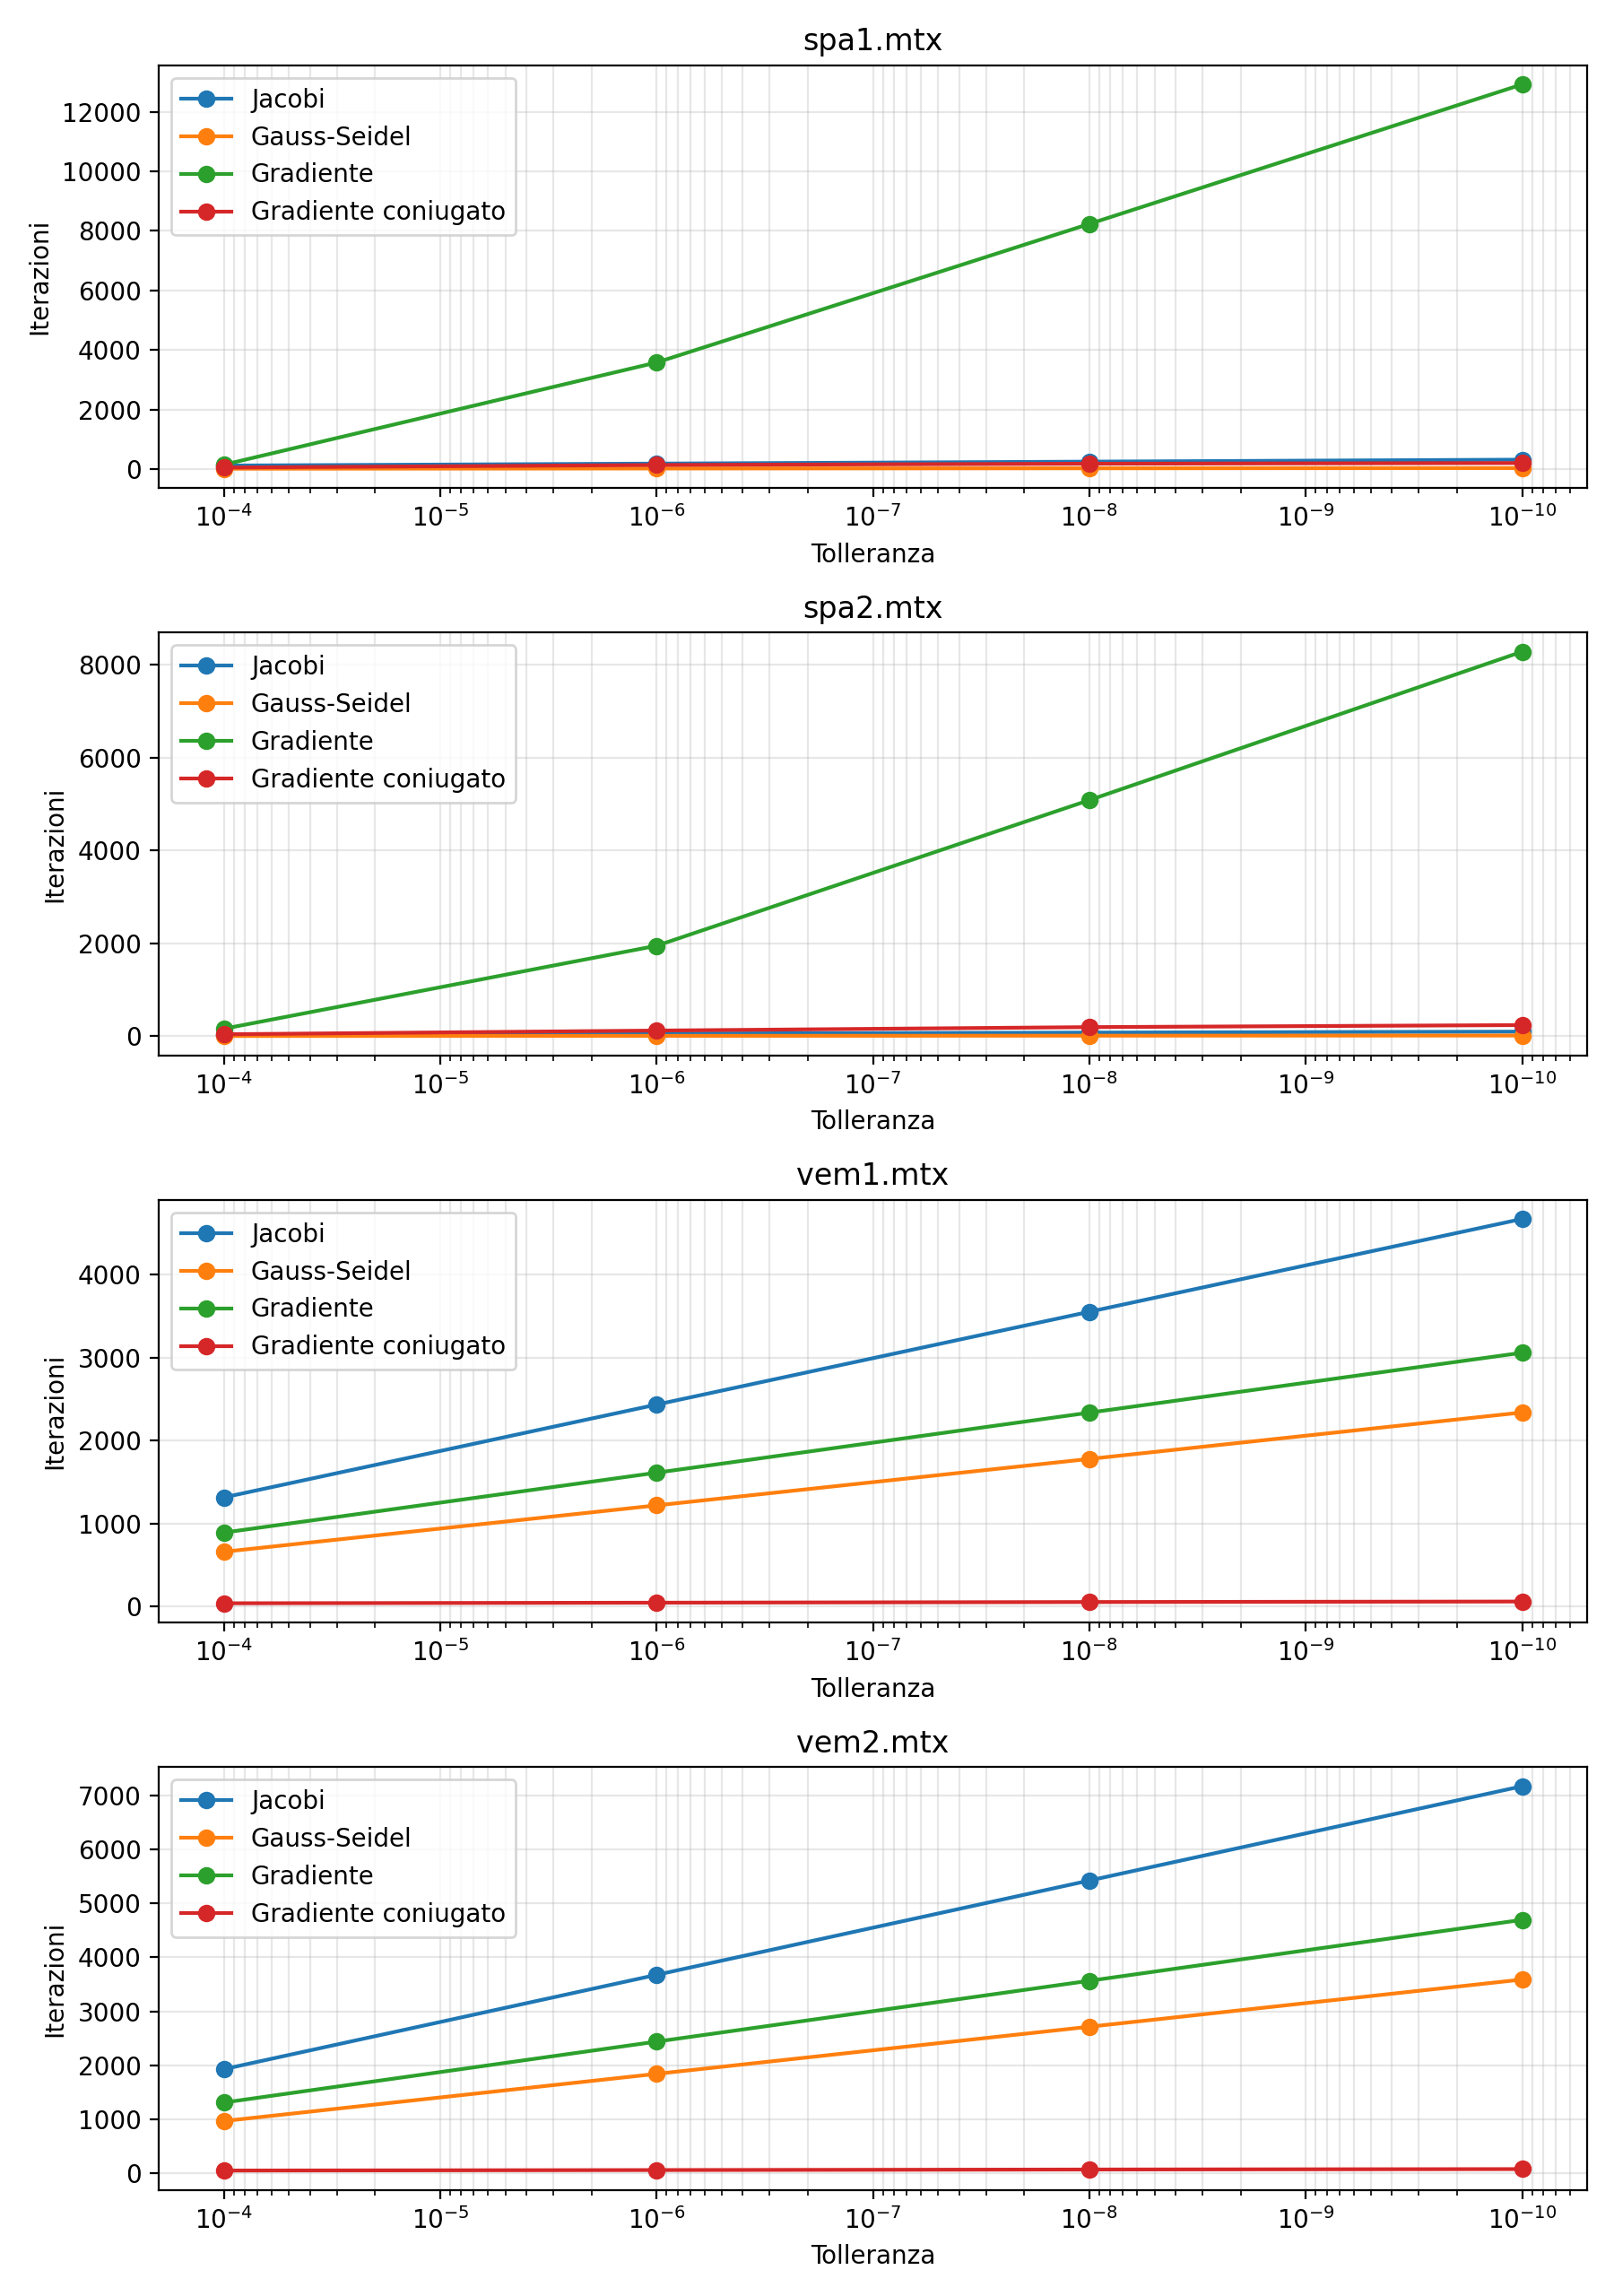
\includegraphics[width=0.72\textwidth]{../results/plots/iterations.png}
\caption{Numero di iterazioni al variare di \texttt{tol} (asse $x$ in scala
logaritmica, una riga per matrice; asse $y$ lineare).}
\label{fig:iter}
\end{figure}

Da un punto di vista teorico, ci si aspetta che il numero di iterazioni dei metodi
stazionari sia governato dalla \emph{dominanza diagonale} (cioè dal raggio
spettrale $\rho(P^{-1}N)$), mentre quello dei metodi del gradiente dipenda dal
\emph{numero di condizionamento}. I risultati sono mostrati nella
Figura~\ref{fig:iter}.

L'osservazione dei risultati conferma queste premesse in maniera esemplare, e
mette in luce due scenari opposti. Sulle \texttt{spa} la curva del Gradiente
\guillemotleft sfonda\guillemotright\ verso l'alto in modo marcato, crescendo quasi
linearmente fino a $12\,919$ iterazioni su \texttt{spa1} e $8\,285$ su \texttt{spa2}
a $\texttt{tol}=10^{-10}$, mentre Jacobi, Gauss--Seidel e Gradiente coniugato
restano schiacciati in basso, indistinguibili a poche centinaia di passi o meno.
Sulle \texttt{vem} lo scenario si capovolge: la curva più alta diventa quella di
Jacobi (fino a $7\,174$ su \texttt{vem2}), seguita dal Gradiente e poi da
Gauss--Seidel --- che ne dimezza con regolarità i passi --- mentre il Gradiente
coniugato si appiattisce su una linea quasi orizzontale di poche decine di
iterazioni. Ci troviamo di fronte alle due leggi annunciate: le \texttt{spa} sono
fortemente dominanti diagonali (stazionari fulminei) ma mal condizionate
(Gradiente lentissimo per via dello \emph{zig-zag}); le \texttt{vem}, meno
dominanti ma meglio condizionate, riequilibrano la gara. In entrambi i regimi il
Gradiente coniugato, che scala come $\sqrt{\mathrm{cond}(A)}$, resta nettamente il
più parsimonioso.

\subsubsection{Errore relativo}
\begin{figure}[H]
\centering
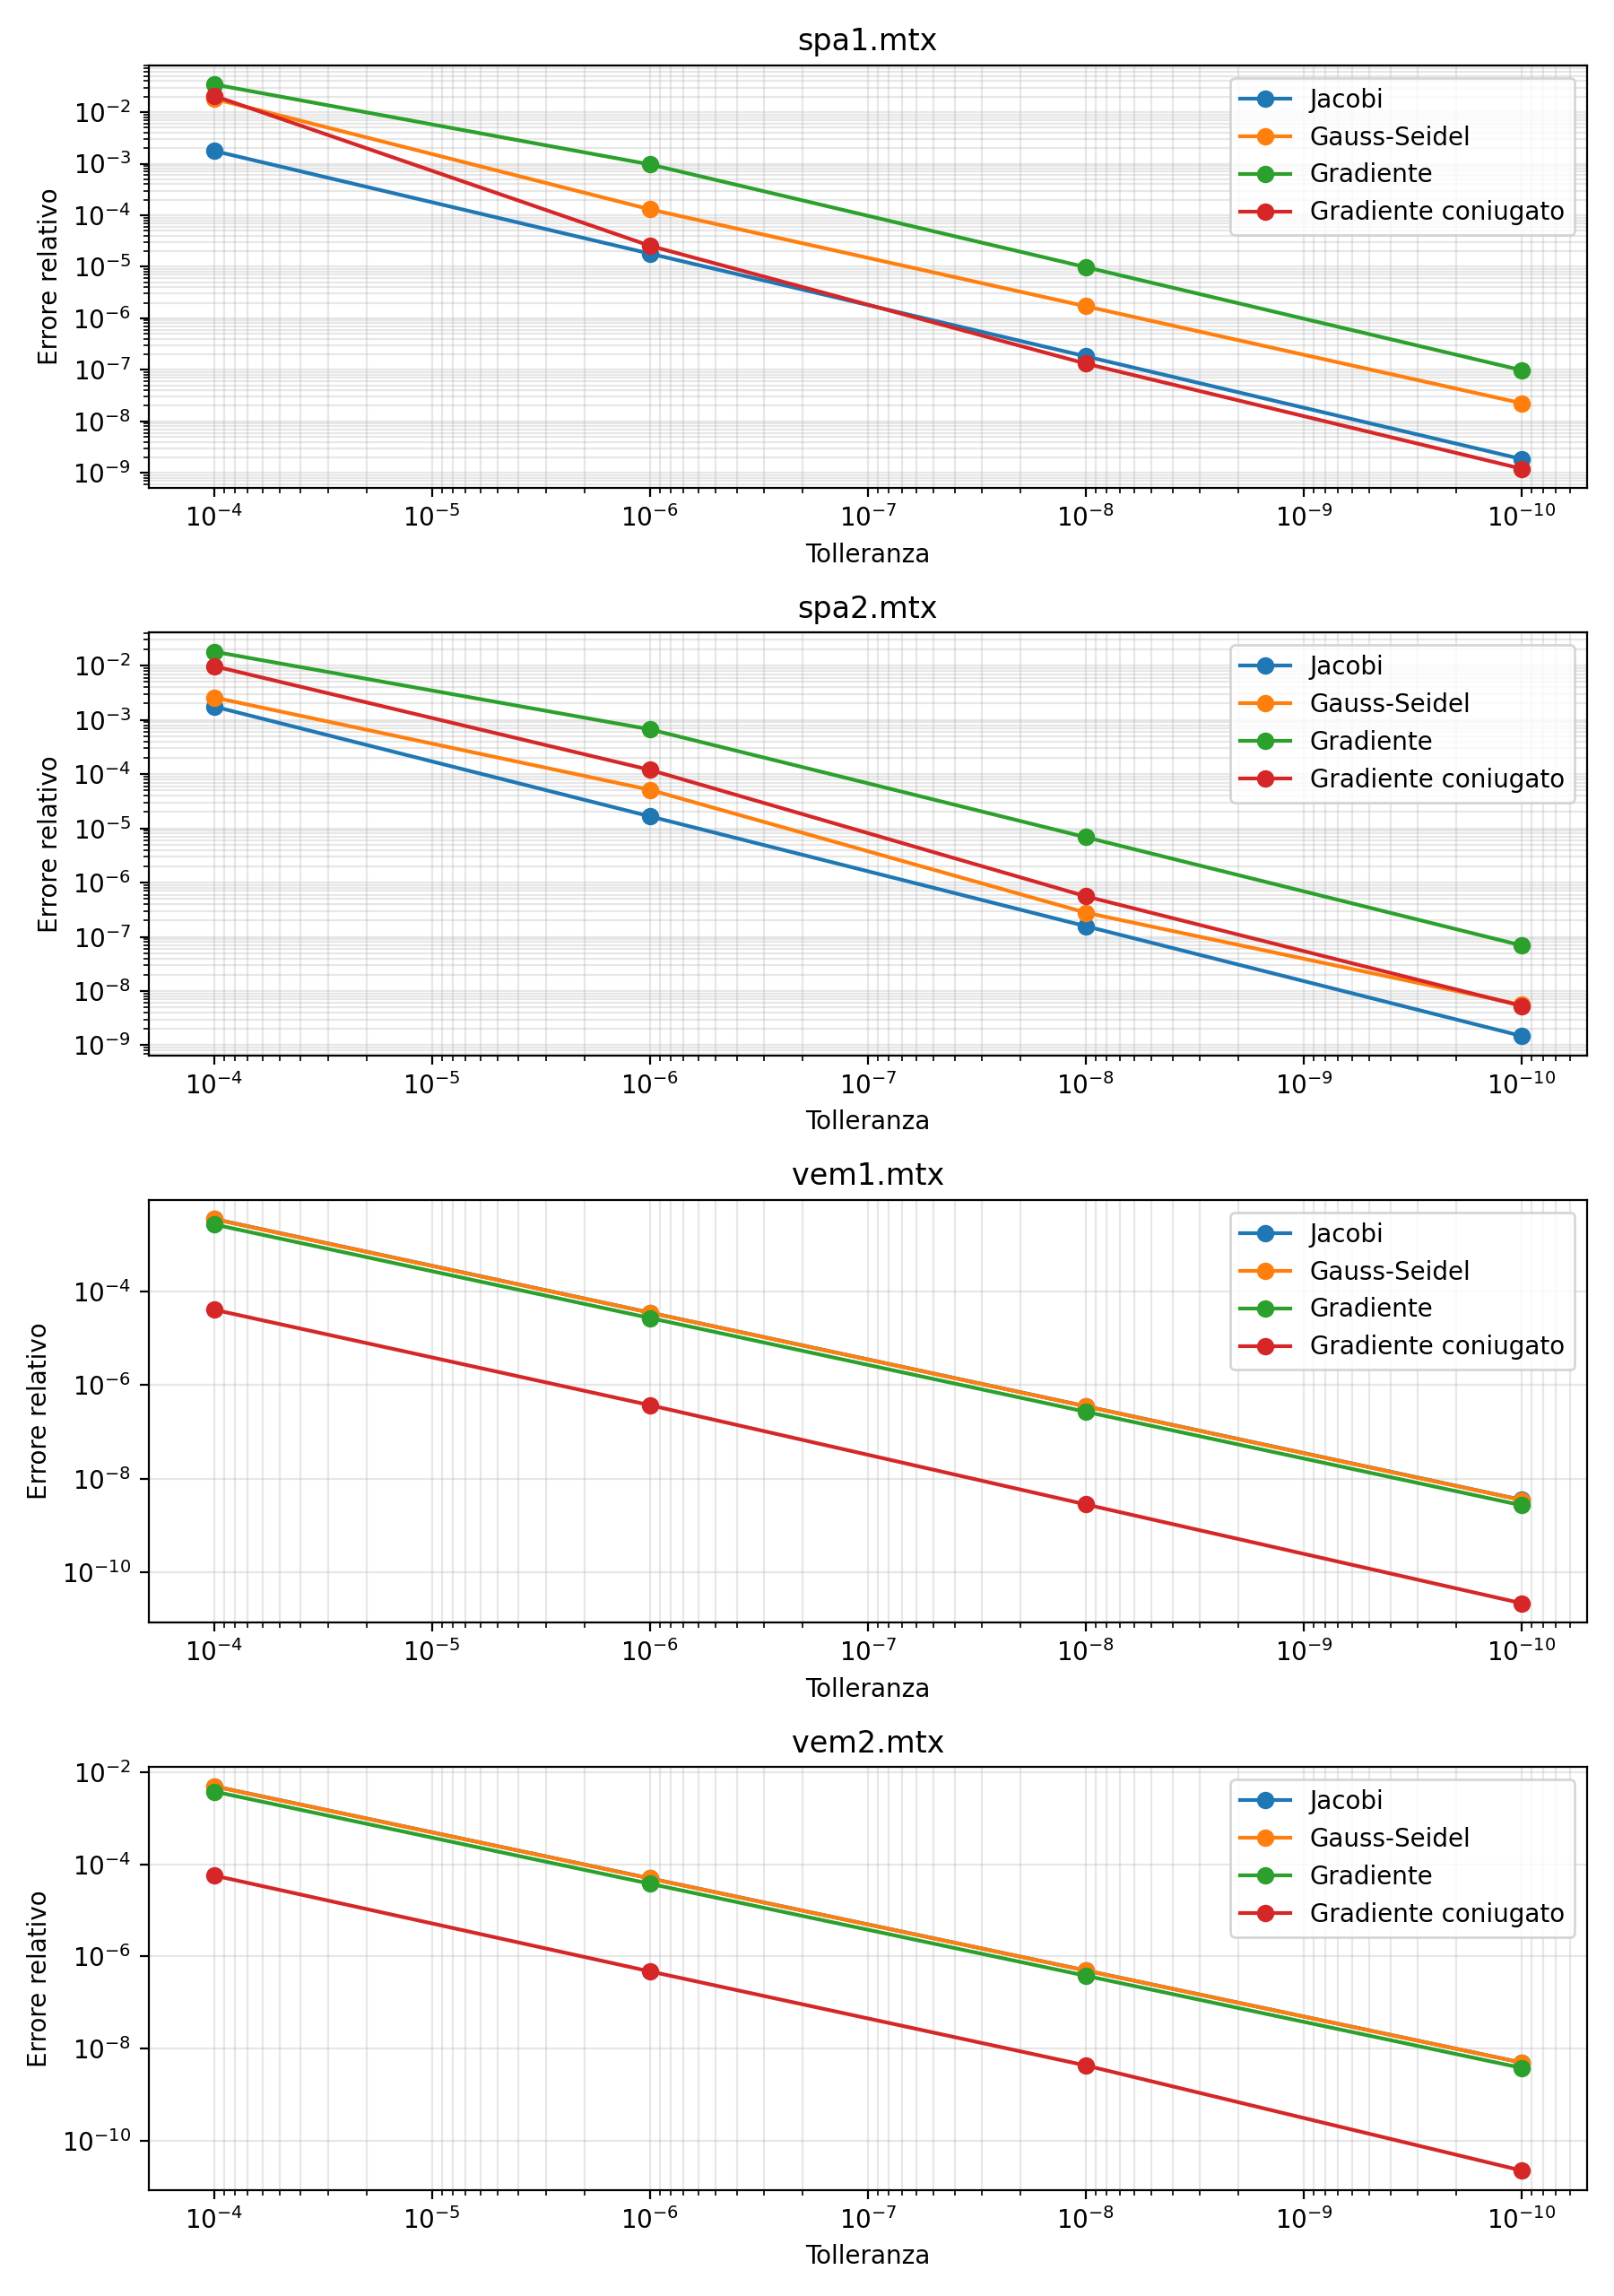
\includegraphics[width=0.72\textwidth]{../results/plots/relative_error.png}
\caption{Errore relativo $\lVert\mathbf{x}_{\text{calc}}-\mathbf{x}\rVert/
\lVert\mathbf{x}\rVert$ al variare di \texttt{tol} (entrambi gli assi in scala
logaritmica, una riga per matrice).}
\label{fig:err}
\end{figure}

Un principio centrale, già richiamato fra i metodi, è che il criterio d'arresto controlla
il \emph{residuo}, non l'errore vero, e che il ponte fra i due è il
condizionamento ($\text{errore}\lesssim\mathrm{cond}(A)\cdot\text{residuo}$). È
prevedibile, di conseguenza, che a parità di tolleranza l'errore non sia lo stesso
fra i metodi. La Figura~\ref{fig:err} riporta l'errore relativo vero
$\lVert\mathbf{x}_{\text{calc}}-\mathbf{x}\rVert/\lVert\mathbf{x}\rVert$.

I risultati convalidano l'assunto di partenza. Tutte le curve scendono in modo
sostanzialmente lineare al ridursi della tolleranza --- un decadimento atteso,
poiché la soglia agisce direttamente sul residuo --- ma la loro \emph{posizione
verticale} racconta il ruolo del condizionamento. Sulle \texttt{spa} il Gradiente
mantiene la curva di errore più alta, mentre Jacobi, Gauss--Seidel e Gradiente
coniugato si collocano più in basso, comunque entro circa un ordine di grandezza
l'una dall'altra. Sulle \texttt{vem} lo scenario è il più eloquente: le curve di
Jacobi, Gauss--Seidel e Gradiente si \textbf{sovrappongono quasi perfettamente},
segno che condividono lo stesso fattore di amplificazione, mentre quella del
Gradiente coniugato corre nettamente al di sotto, $1$--$2$ ordini di grandezza più
in basso. Ad esempio a $\texttt{tol}=10^{-10}$ su \texttt{vem1}, dove gli altri tre
si fermano a $\sim$$3.5\cdot10^{-9}$, il Gradiente coniugato raggiunge
$2.19\cdot10^{-11}$, un errore addirittura inferiore al residuo imposto. La
spiegazione è che il Gradiente coniugato non si limita a inseguire la componente
dominante dell'errore, ma tende ad abbattere simultaneamente tutte le componenti
spettrali: a parità di residuo, restituisce la soluzione più accurata.

\subsubsection{Tempo di calcolo}
\begin{figure}[H]
\centering
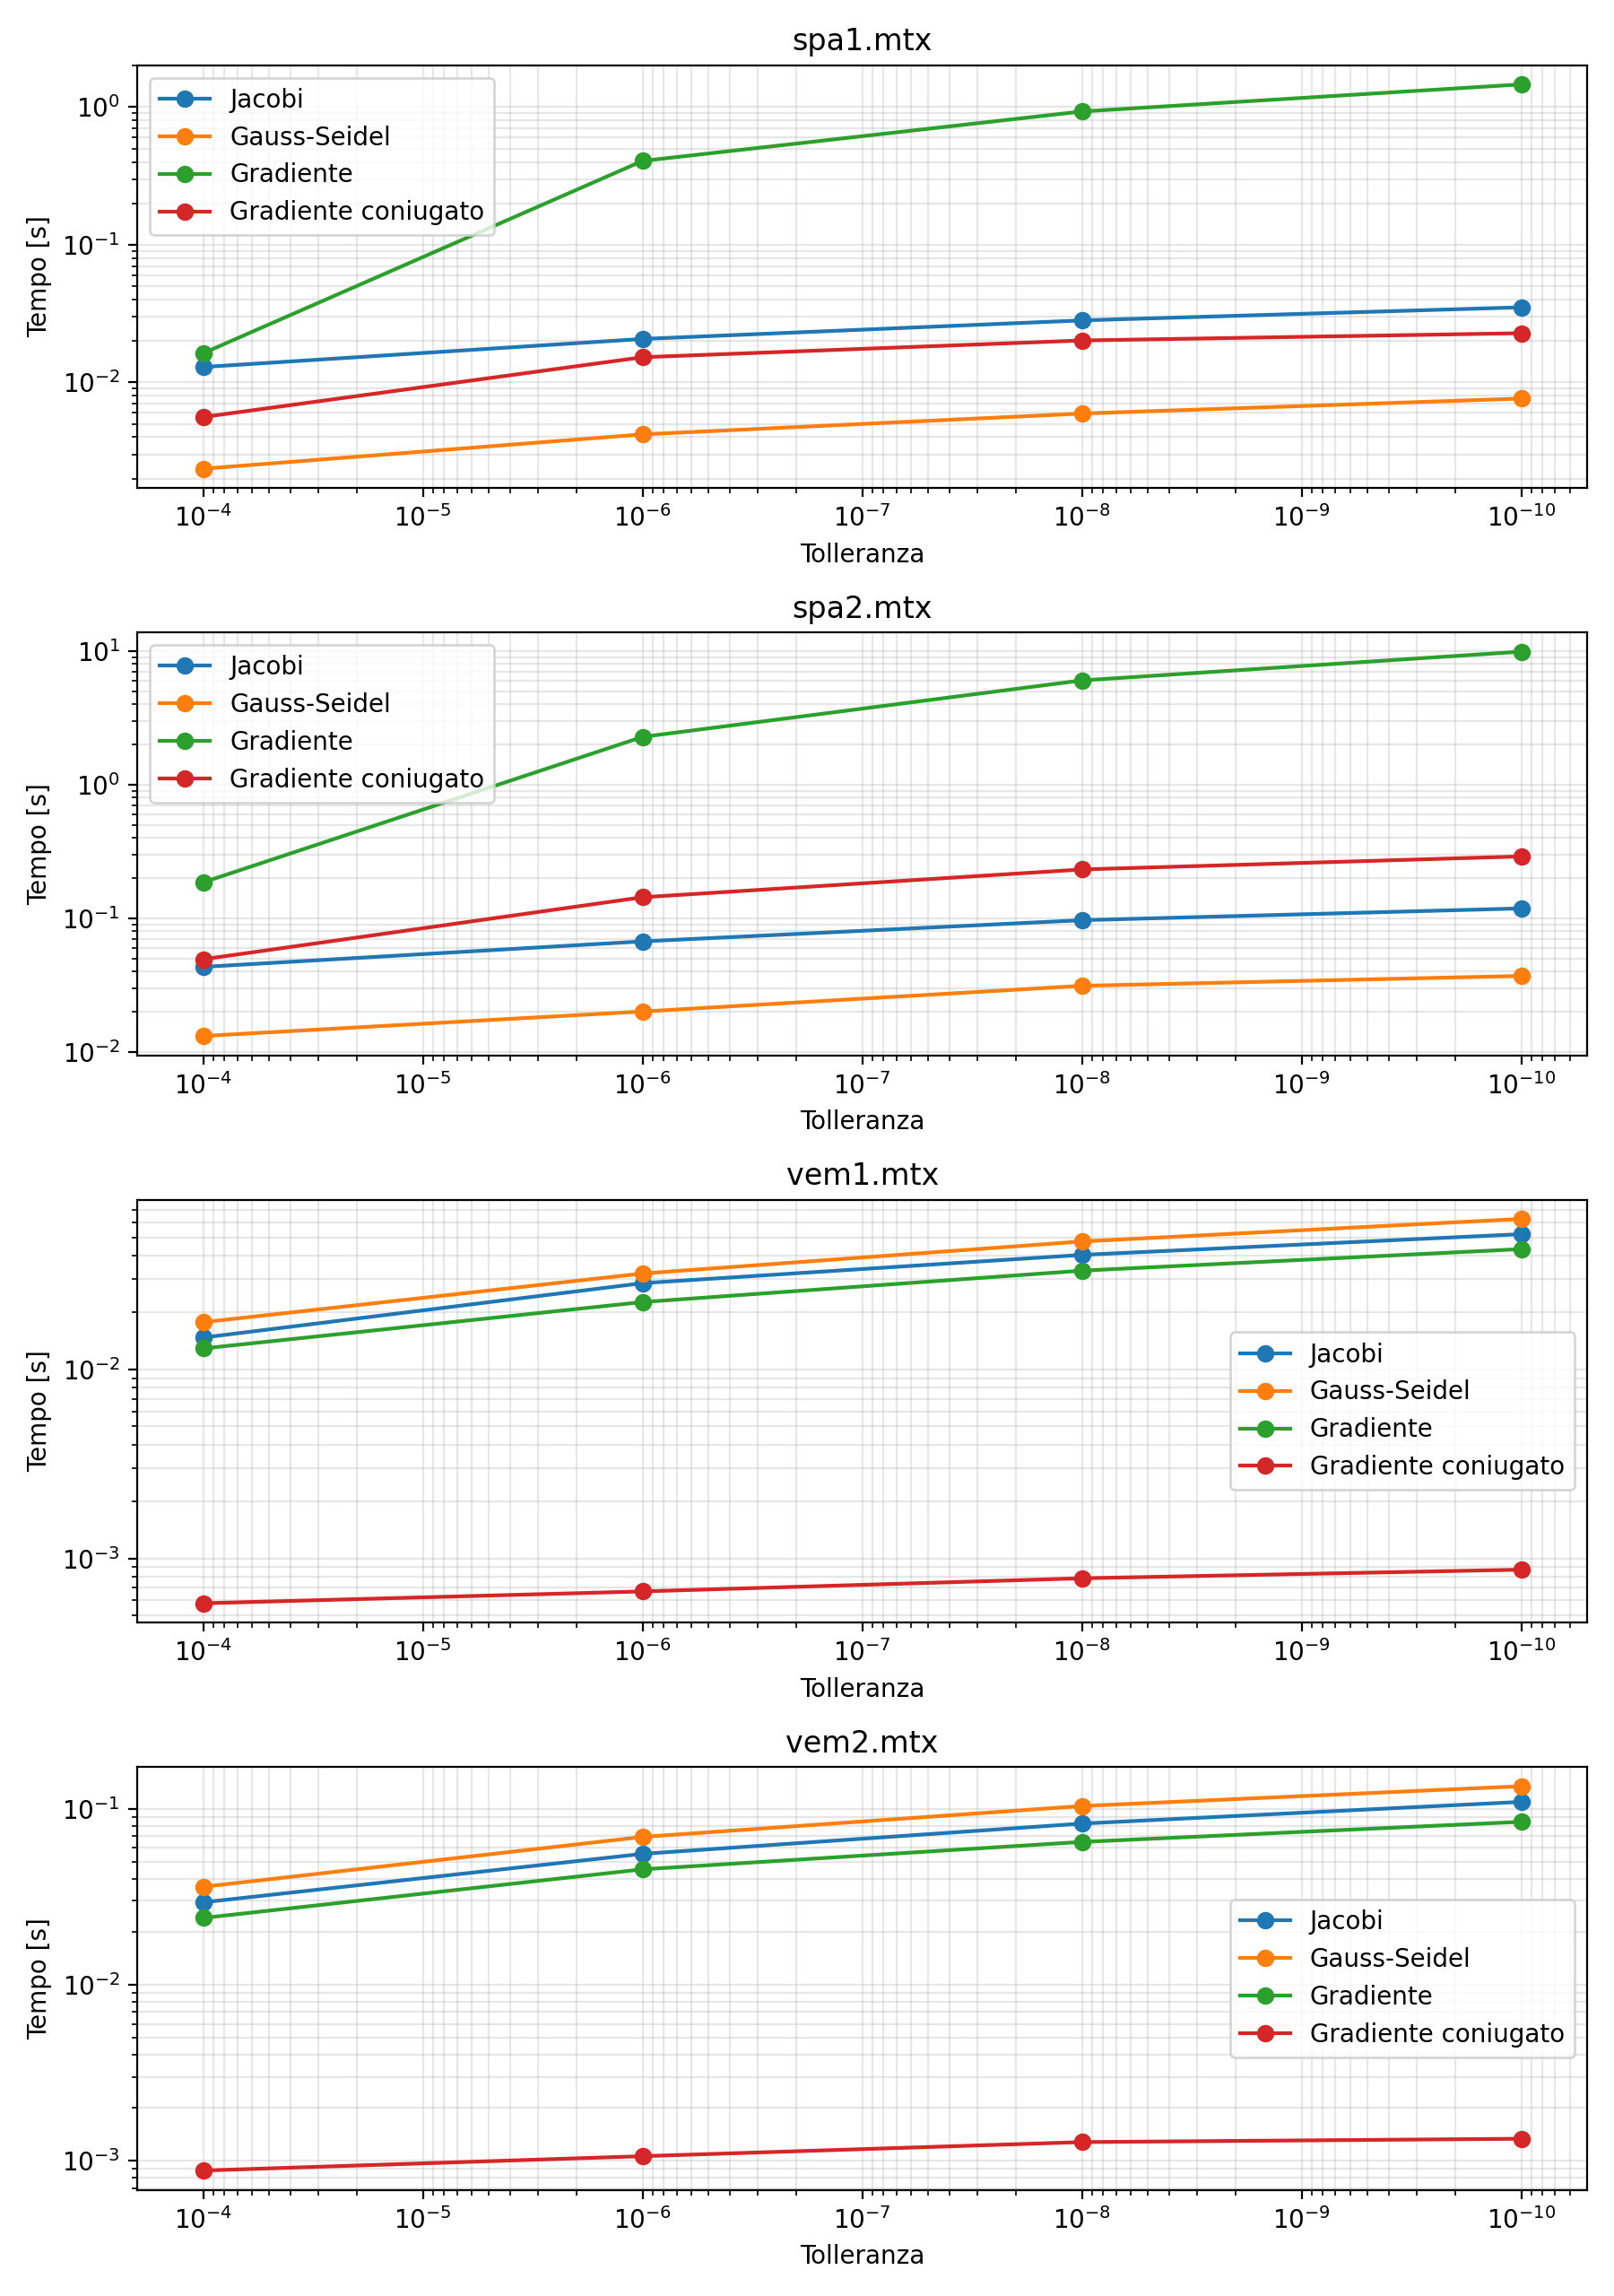
\includegraphics[width=0.72\textwidth]{../results/plots/time.png}
\caption{Tempo di calcolo al variare di \texttt{tol} (asse $y$ in scala
logaritmica, una riga per matrice).}
\label{fig:time}
\end{figure}

Il tempo totale è il prodotto di due fattori --- il \emph{numero di iterazioni} e
il \emph{costo del singolo passo} --- e quest'ultimo, dominato dal prodotto
matrice--vettore, cresce con il numero di non-zeri della matrice. Trattandosi di
densità molto diverse fra le due famiglie, è prevedibile uno scenario meno
uniforme dei precedenti. I tempi misurati sono riportati nella
Figura~\ref{fig:time}.

L'osservazione conferma queste premesse. Sulle \texttt{spa}, dense e quindi con
\emph{matvec} costoso, il prezzo delle molte iterazioni del Gradiente diventa
severo: la sua curva sale isolata in cima, fino a $9.89$\,s su \texttt{spa2} a
$\texttt{tol}=10^{-10}$, contro i $0.037$\,s di Gauss--Seidel --- la curva più
bassa, grazie al numero ridottissimo di passi --- e i $0.291$\,s del Gradiente
coniugato. Sulle \texttt{vem}, molto sparse e quindi con passo economico, le tre
curve di Jacobi, Gauss--Seidel e Gradiente si addensano in alto attorno a
$0.05$--$0.13$\,s, mentre il Gradiente coniugato corre per distacco al di sotto, su
valori dell'ordine di $10^{-3}$\,s. In altri termini, dove il costo per iterazione
è alto vince chi fa meno iterazioni \emph{utili} (Gauss--Seidel sulle \texttt{spa},
nonostante la \emph{sweep} sequenziale); dove è basso, il tempo segue da vicino il
numero di iterazioni, e il Gradiente coniugato domina senza rivali.

\clearpage
\subsection{Grafici di approfondimento}
Ai tre grafici fondamentali abbiamo affiancato cinque ulteriori figure (script
\texttt{plots.py}), ciascuna costruita per isolare un aspetto che la lettura
\guillemotleft metrica vs tolleranza\guillemotright\ lascia in ombra: la dinamica
iterazione per iterazione, la dipendenza esplicita dal condizionamento,
l'amplificazione dell'errore e la scomposizione del tempo nei suoi due fattori.

\subsubsection{Storia di convergenza}
\begin{figure}[H]
\centering
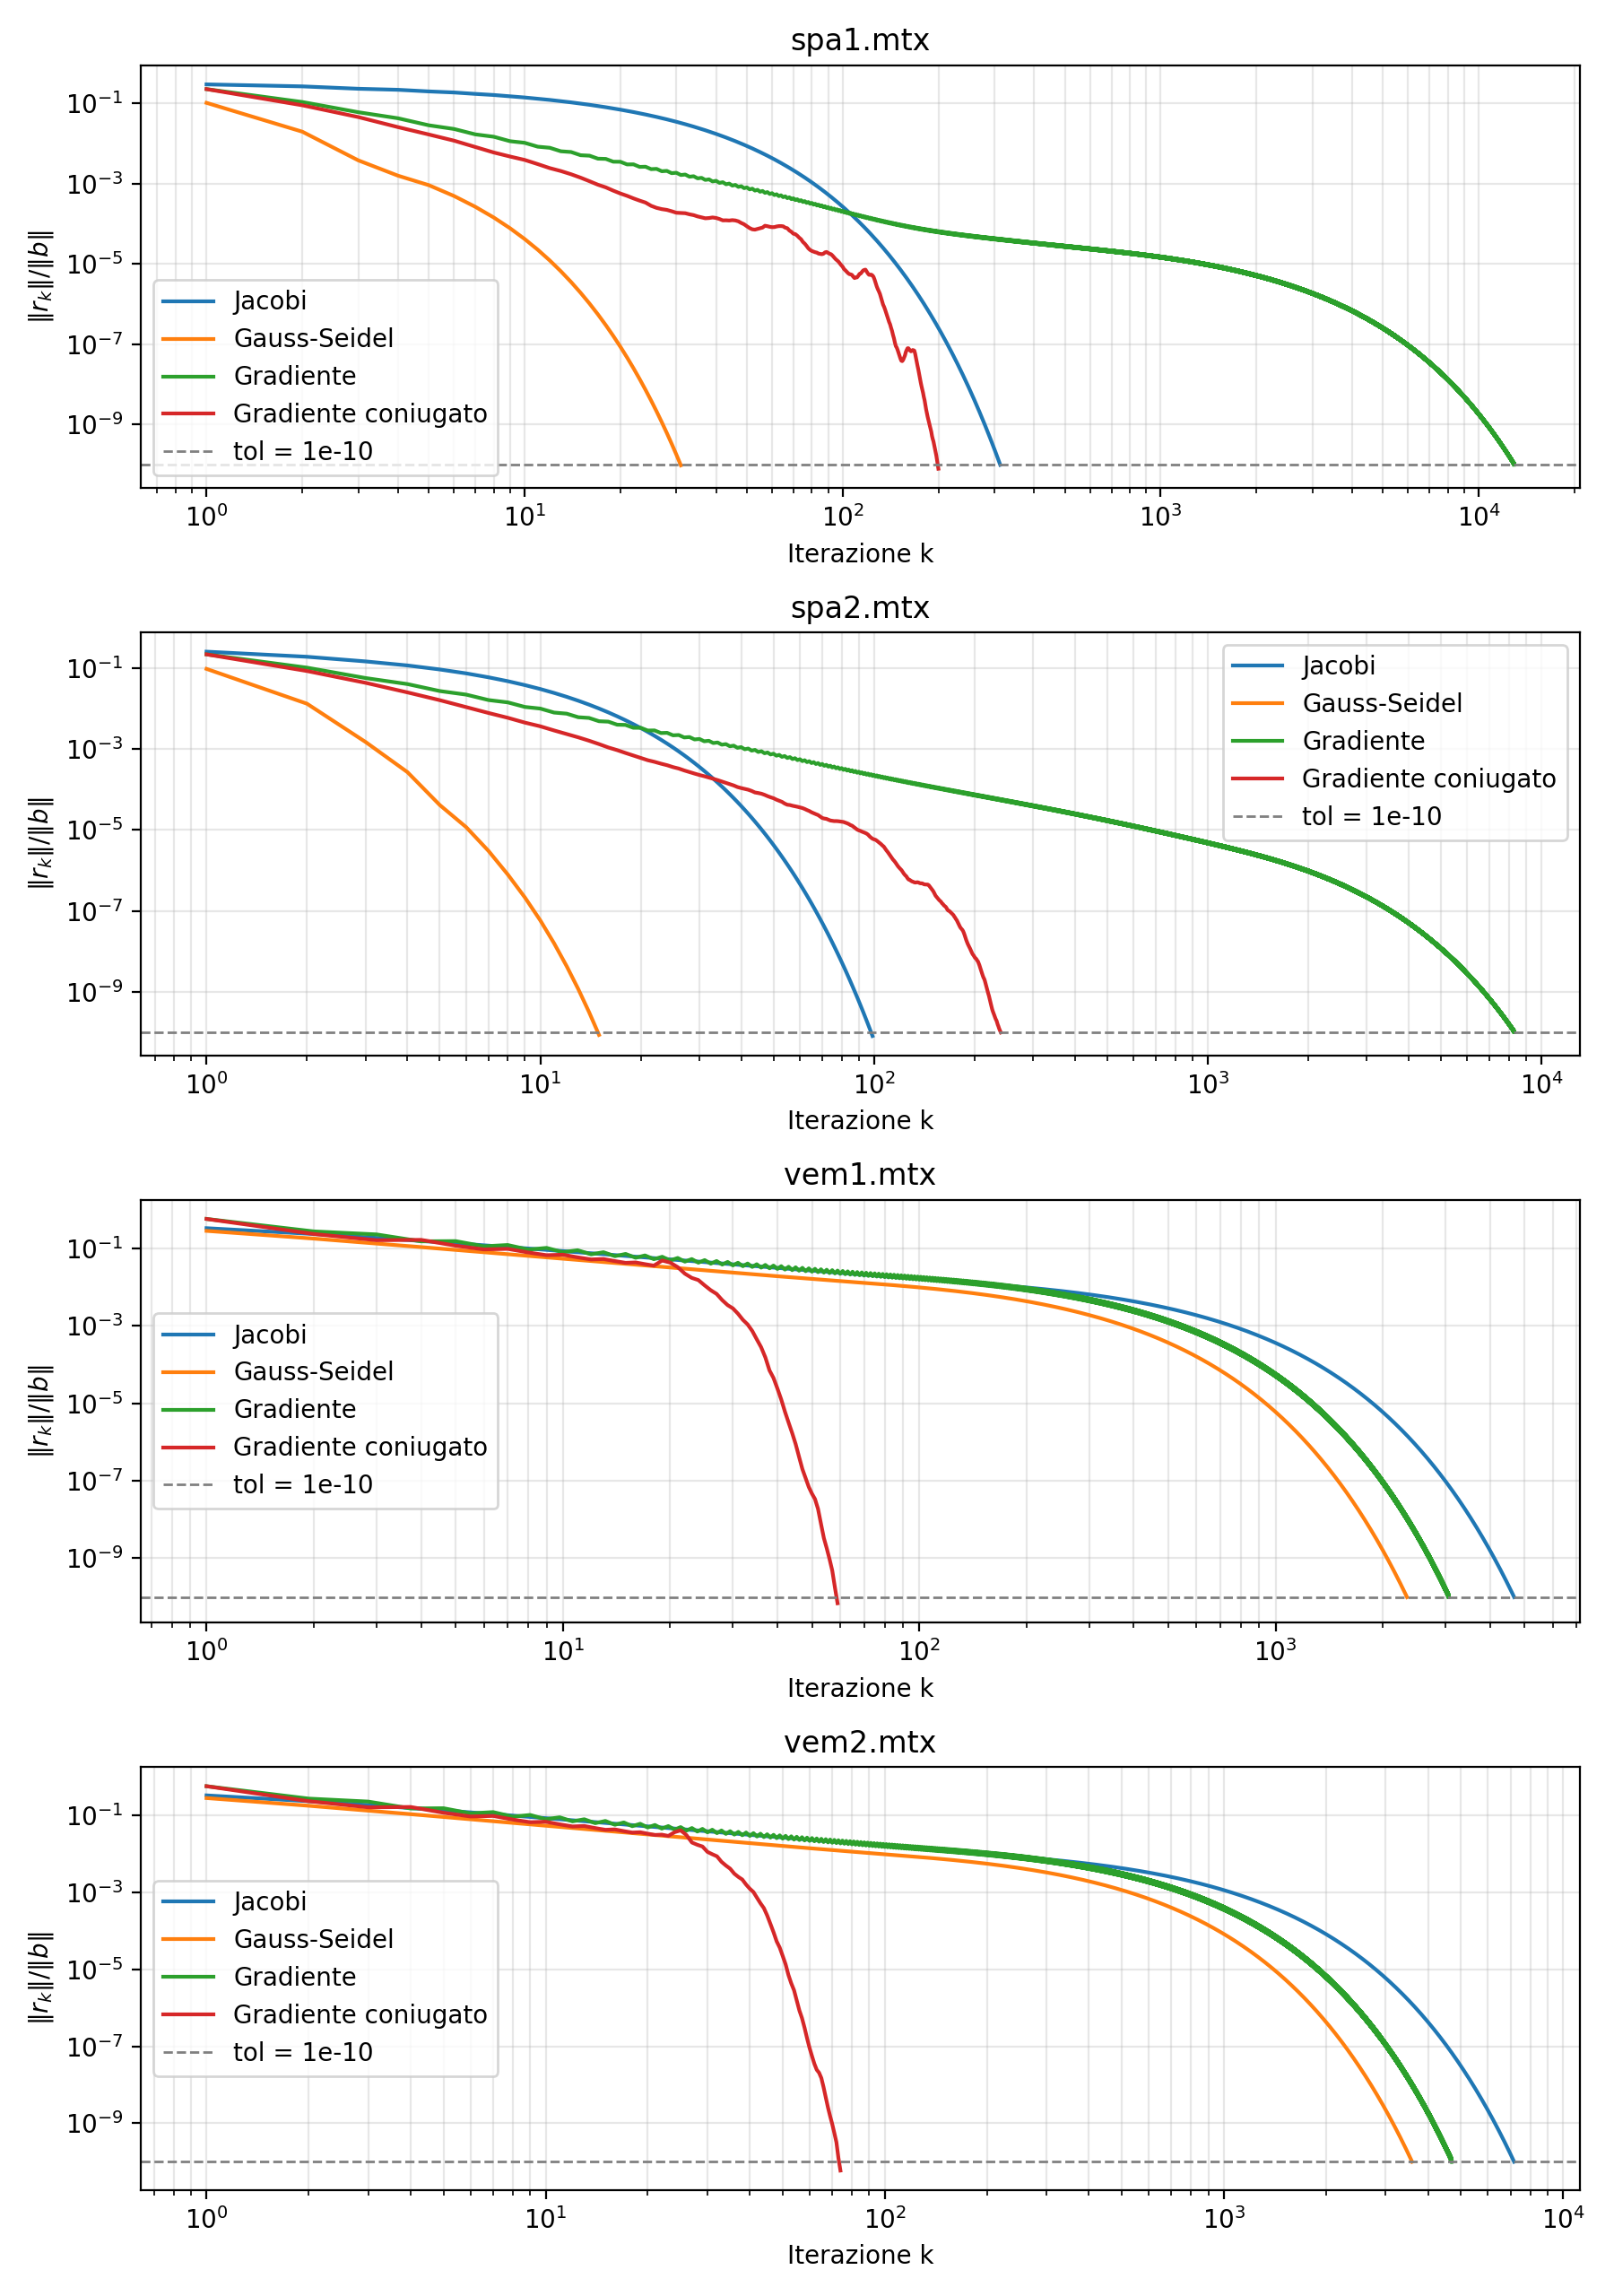
\includegraphics[width=0.74\textwidth]{../results/plots/convergence.png}
\caption{Storia del residuo scalato $\lVert\mathbf{r}_k\rVert/\lVert\mathbf{b}\rVert$
in funzione dell'iterazione $k$ (\texttt{tol}$=10^{-10}$, entrambi gli assi in scala
logaritmica, una riga per matrice; la linea tratteggiata segna la tolleranza).}
\label{fig:conv}
\end{figure}

Da un punto di vista teorico, ci si aspetta che ogni famiglia di metodi lasci una
\guillemotleft firma\guillemotright\ riconoscibile nella discesa del residuo: un
decadimento lineare (in scala semilogaritmica) per i metodi stazionari, un profilo
irregolare e lento per il Gradiente sulle matrici mal condizionate, una caduta
superlineare per il Gradiente coniugato. La storia del residuo scalato in funzione
dell'iterazione è riportata nella Figura~\ref{fig:conv}.

L'osservazione dei risultati conferma queste premesse in maniera esemplare. Le
curve di Jacobi e Gauss--Seidel scendono come rette, con quella di Gauss--Seidel
sistematicamente più ripida; il Gradiente, sulle \texttt{spa}, procede invece a
\guillemotleft gradoni\guillemotright\ e si trascina per migliaia di iterazioni
prima di toccare la soglia, mentre il Gradiente coniugato precipita e taglia la
linea della tolleranza in poche decine di passi. Questo si verifica poiché le
direzioni $A$-coniugate non disfanno il lavoro già compiuto: ogni passo abbatte una
componente dell'errore senza riaprirne altre, laddove il Gradiente semplice, nella
valle stretta delle matrici mal condizionate, rimbalza da una parete all'altra. La
\emph{firma} grafica dei tre comportamenti coincide con la previsione teorica.

\subsubsection{Iterazioni e numero di condizionamento}
\begin{figure}[H]
\centering
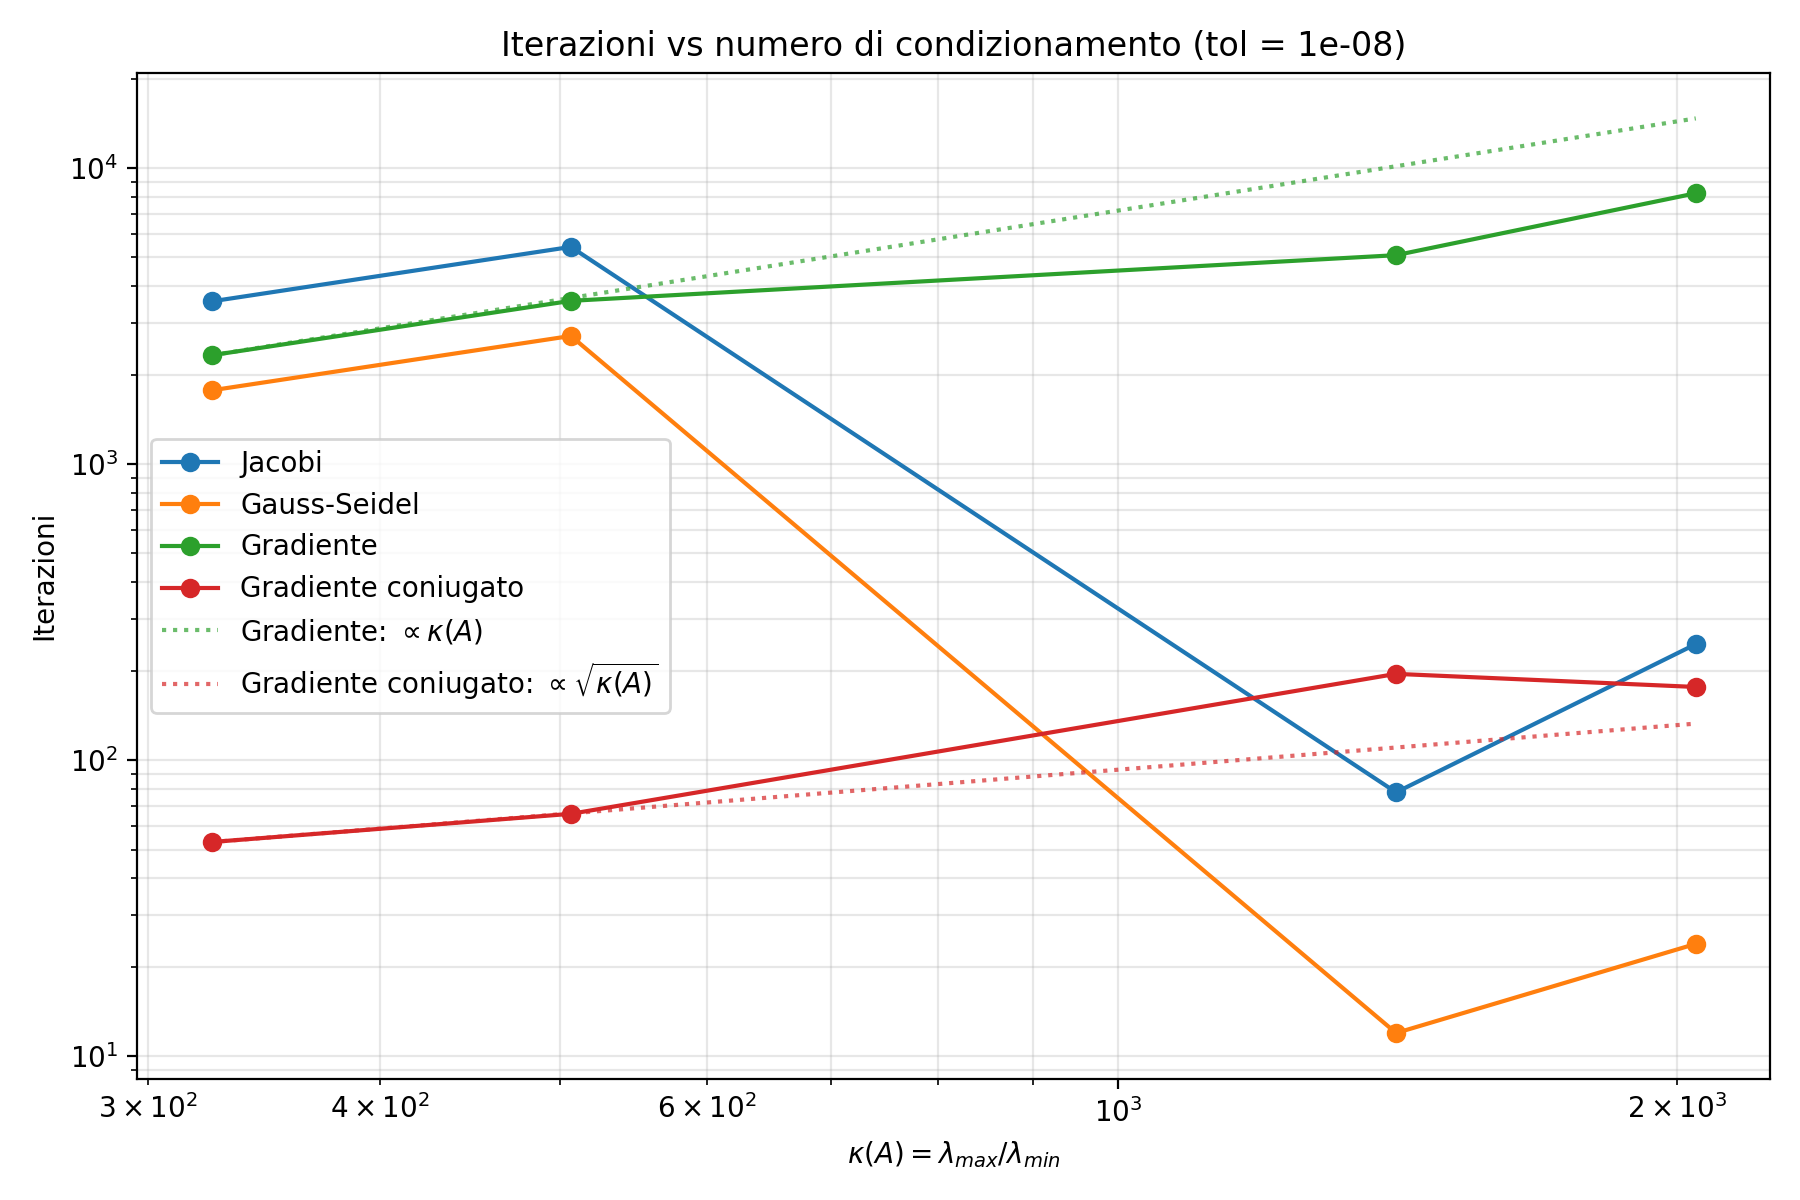
\includegraphics[width=0.74\textwidth]{../results/plots/iter_vs_cond.png}
\caption{Iterazioni in funzione di $\mathrm{cond}(A)$ (\texttt{tol}$=10^{-8}$, assi
logaritmici), con le curve teoriche $\propto\kappa(A)$ (Gradiente) e
$\propto\sqrt{\kappa(A)}$ (Gradiente coniugato) ancorate al dato a condizionamento
minimo.}
\label{fig:itercond}
\end{figure}

Un principio centrale già introdotto lega il numero di iterazioni del Gradiente al
condizionamento ($\propto\kappa(A)$) e quello del Gradiente coniugato alla sua
radice ($\propto\sqrt{\kappa(A)}$), mentre i metodi stazionari restano governati
dalla dominanza diagonale e non dal condizionamento. Per metterlo alla prova
abbiamo riportato le iterazioni in funzione di $\mathrm{cond}(A)$, affiancando le
due curve teoriche di riferimento, nella Figura~\ref{fig:itercond}.

L'andamento sperimentale rispetta le predizioni teoriche. I punti del Gradiente si
dispongono lungo la curva ripida $\propto\kappa(A)$, quelli del Gradiente coniugato
lungo la più dolce $\propto\sqrt{\kappa(A)}$; in altri termini, passando da
\texttt{vem1} ($\mathrm{cond}\approx3\cdot10^{2}$) a \texttt{spa1}
($\mathrm{cond}\approx2\cdot10^{3}$) il Gradiente coniugato cresce nettamente meno
del Gradiente. Al contrario, le spezzate di Jacobi e Gauss--Seidel non seguono
alcuna tendenza monotona rispetto a $\mathrm{cond}(A)$ e anzi si incrociano con le
altre: il loro costo non è dettato dal condizionamento, ma dalla dominanza
diagonale. Ci troviamo così di fronte alla conferma visiva delle \guillemotleft due
leggi\guillemotright\ che governano le due famiglie.

\subsubsection{Amplificazione errore/residuo}
\begin{figure}[H]
\centering
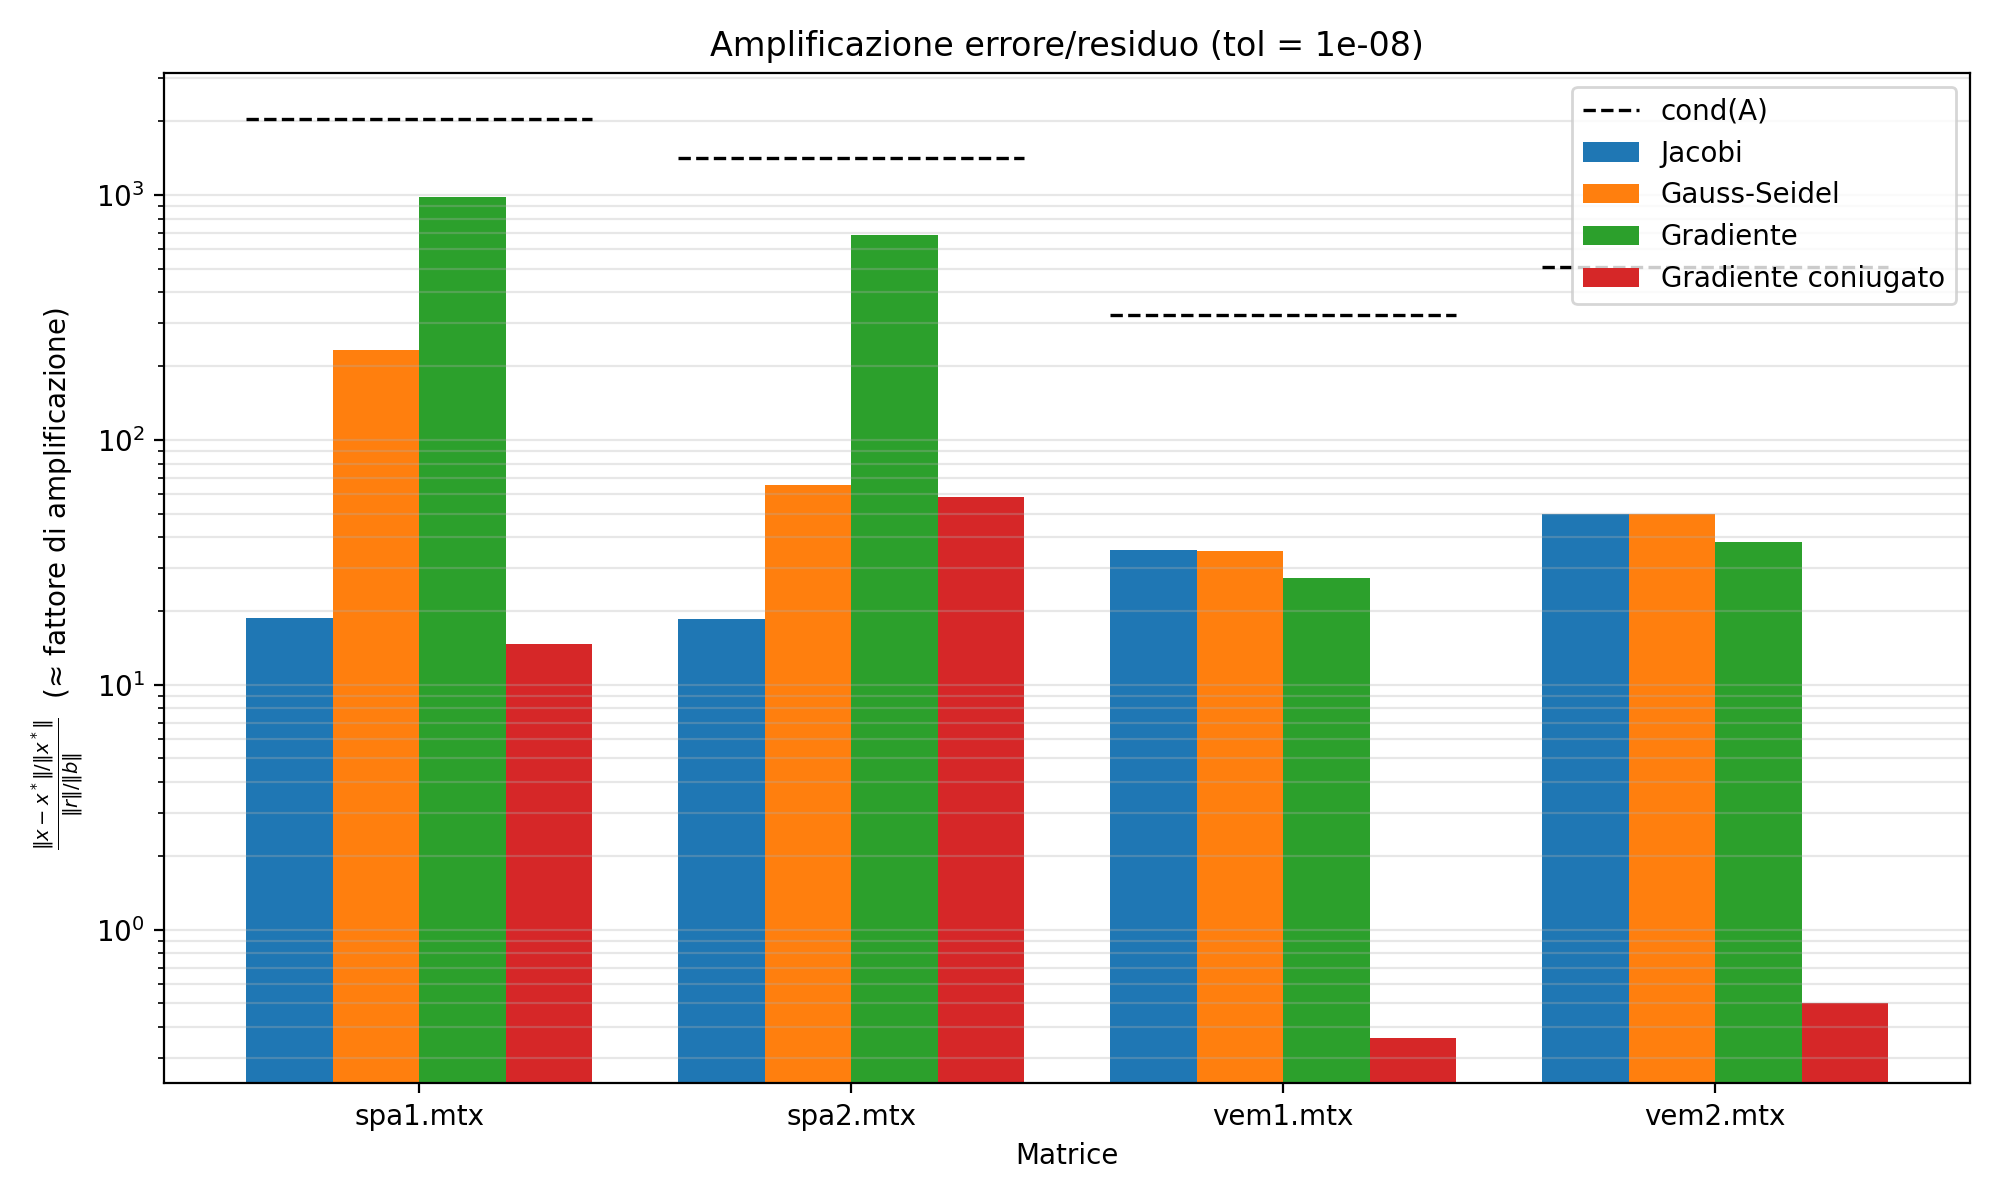
\includegraphics[width=0.74\textwidth]{../results/plots/error_vs_residual.png}
\caption{Fattore di amplificazione errore/residuo per metodo e matrice
(\texttt{tol}$=10^{-8}$, asse $y$ logaritmico); la linea tratteggiata è
$\mathrm{cond}(A)$, limite superiore teorico.}
\label{fig:erramp}
\end{figure}

È prevedibile, dalla relazione $\text{errore}\lesssim\mathrm{cond}(A)\cdot
\text{residuo}$, che il rapporto fra errore vero e residuo scalato resti limitato
superiormente dal \textbf{numero di condizionamento}. La
Figura~\ref{fig:erramp} riporta tale rapporto, metodo per metodo, con la linea
tratteggiata che segna $\mathrm{cond}(A)$ di ciascuna matrice.

I risultati convalidano l'assunto di partenza: in ogni gruppo le barre restano al
di sotto della linea di $\mathrm{cond}(A)$, senza mai violarne il limite. Il
fattore di amplificazione, tuttavia, cambia in maniera marcata fra i metodi: su
\texttt{spa1} il Gradiente amplifica il residuo di circa $9.8\cdot10^{2}$ volte,
quasi al soffitto di $\mathrm{cond}\approx2\cdot10^{3}$, mentre il Gradiente
coniugato si ferma a un fattore di circa $15$. Degno di nota è il caso delle
\texttt{vem}, dove la barra del Gradiente coniugato scende \emph{sotto} l'unità (su
\texttt{vem1} il rapporto vale circa $0.36$): l'errore vero è in quel caso più
piccolo del residuo imposto. In altri termini, a parità di tolleranza il Gradiente
coniugato non solo converge prima, ma restituisce anche la soluzione più fedele.

\subsubsection{Sintesi di tempo e iterazioni}
\begin{figure}[H]
\centering
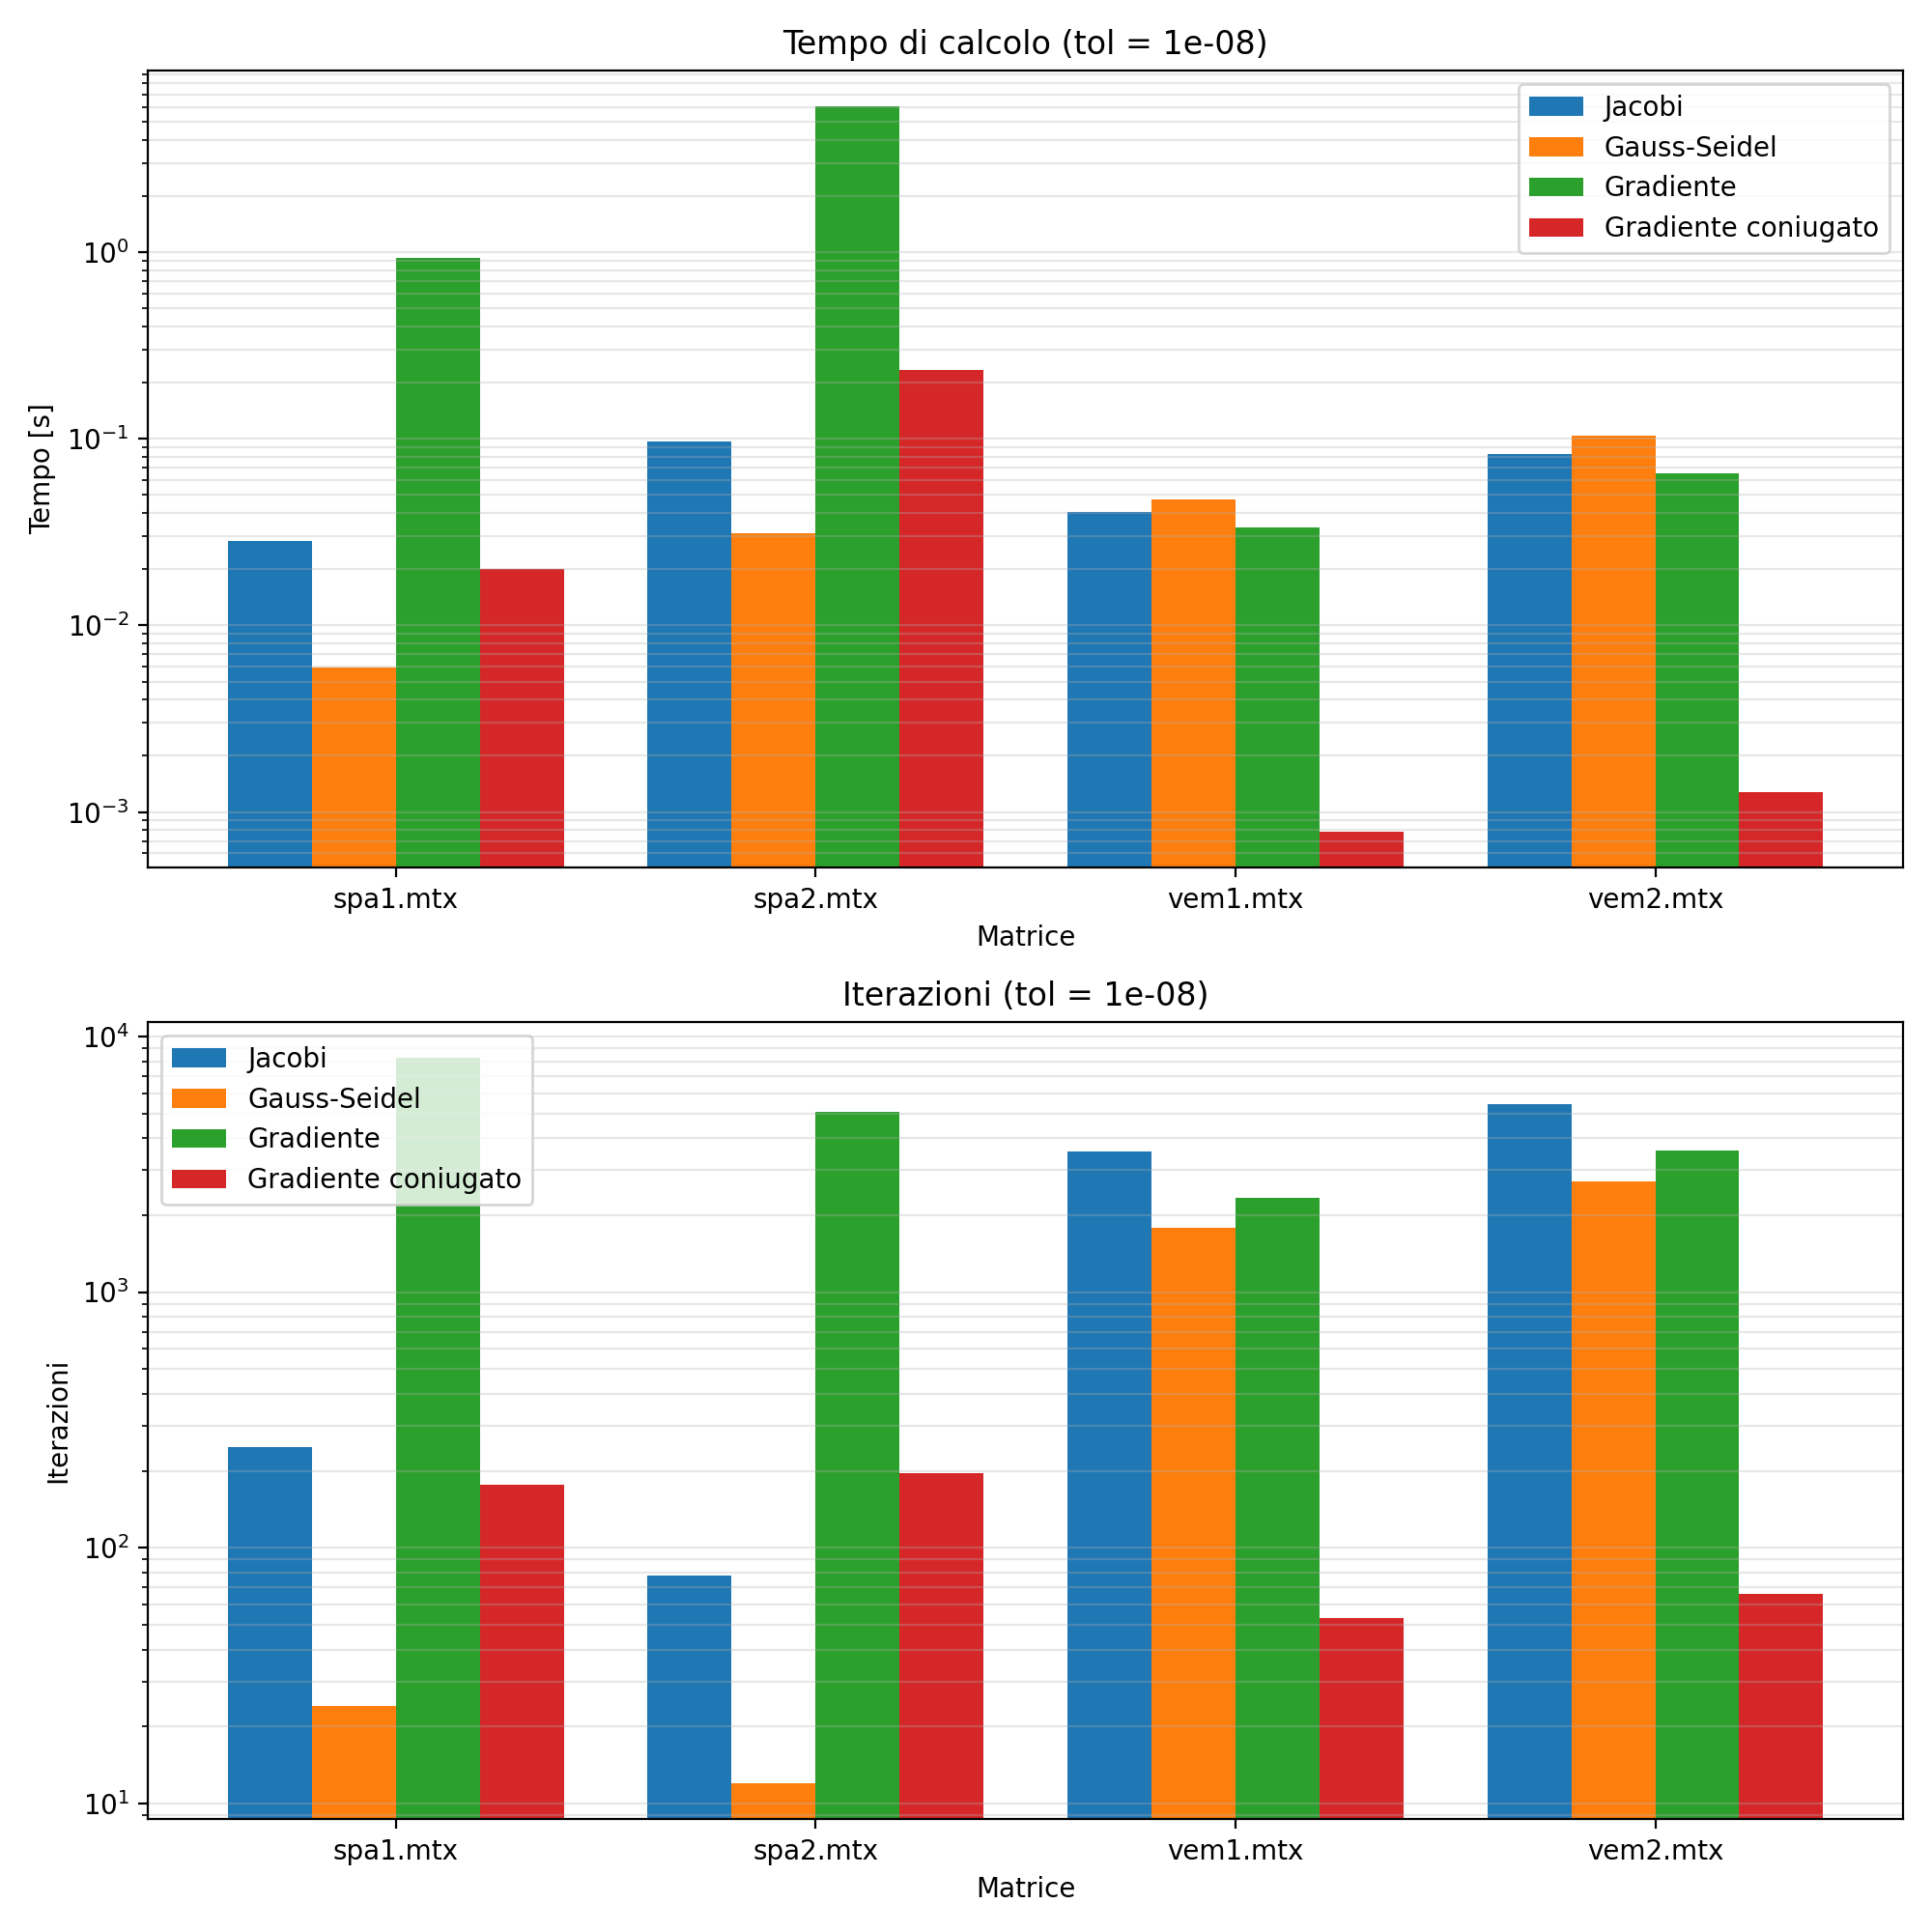
\includegraphics[width=0.78\textwidth]{../results/plots/summary_bars.png}
\caption{Tempo di calcolo (in alto) e numero di iterazioni (in basso) per metodo e
matrice (\texttt{tol}$=10^{-8}$, asse $y$ logaritmico).}
\label{fig:summary}
\end{figure}

Per consolidare in un solo sguardo le curve \guillemotleft metrica vs
tolleranza\guillemotright\ abbiamo fissato una tolleranza rappresentativa e posto a
confronto diretto, a barre, tempo e iterazioni dei quattro metodi. Il quadro è
riportato nella Figura~\ref{fig:summary}.

L'istantanea conferma i due regimi già descritti e li rende immediatamente
confrontabili. Sulle \texttt{spa} la coppia di barre del Gradiente svetta sia in
iterazioni sia in tempo, mentre Gauss--Seidel resta la più bassa; sulle \texttt{vem}
le barre di Jacobi, Gauss--Seidel e Gradiente si allineano su valori simili e quella
del Gradiente coniugato sprofonda, sproporzionalmente più in tempo che in
iterazioni. Questo si verifica poiché il \emph{matvec} sulle \texttt{vem} è
economico: il tempo segue allora da vicino il conteggio dei passi, premiando il
metodo che ne richiede di meno.

\subsubsection{Costo per iterazione}
\begin{figure}[H]
\centering
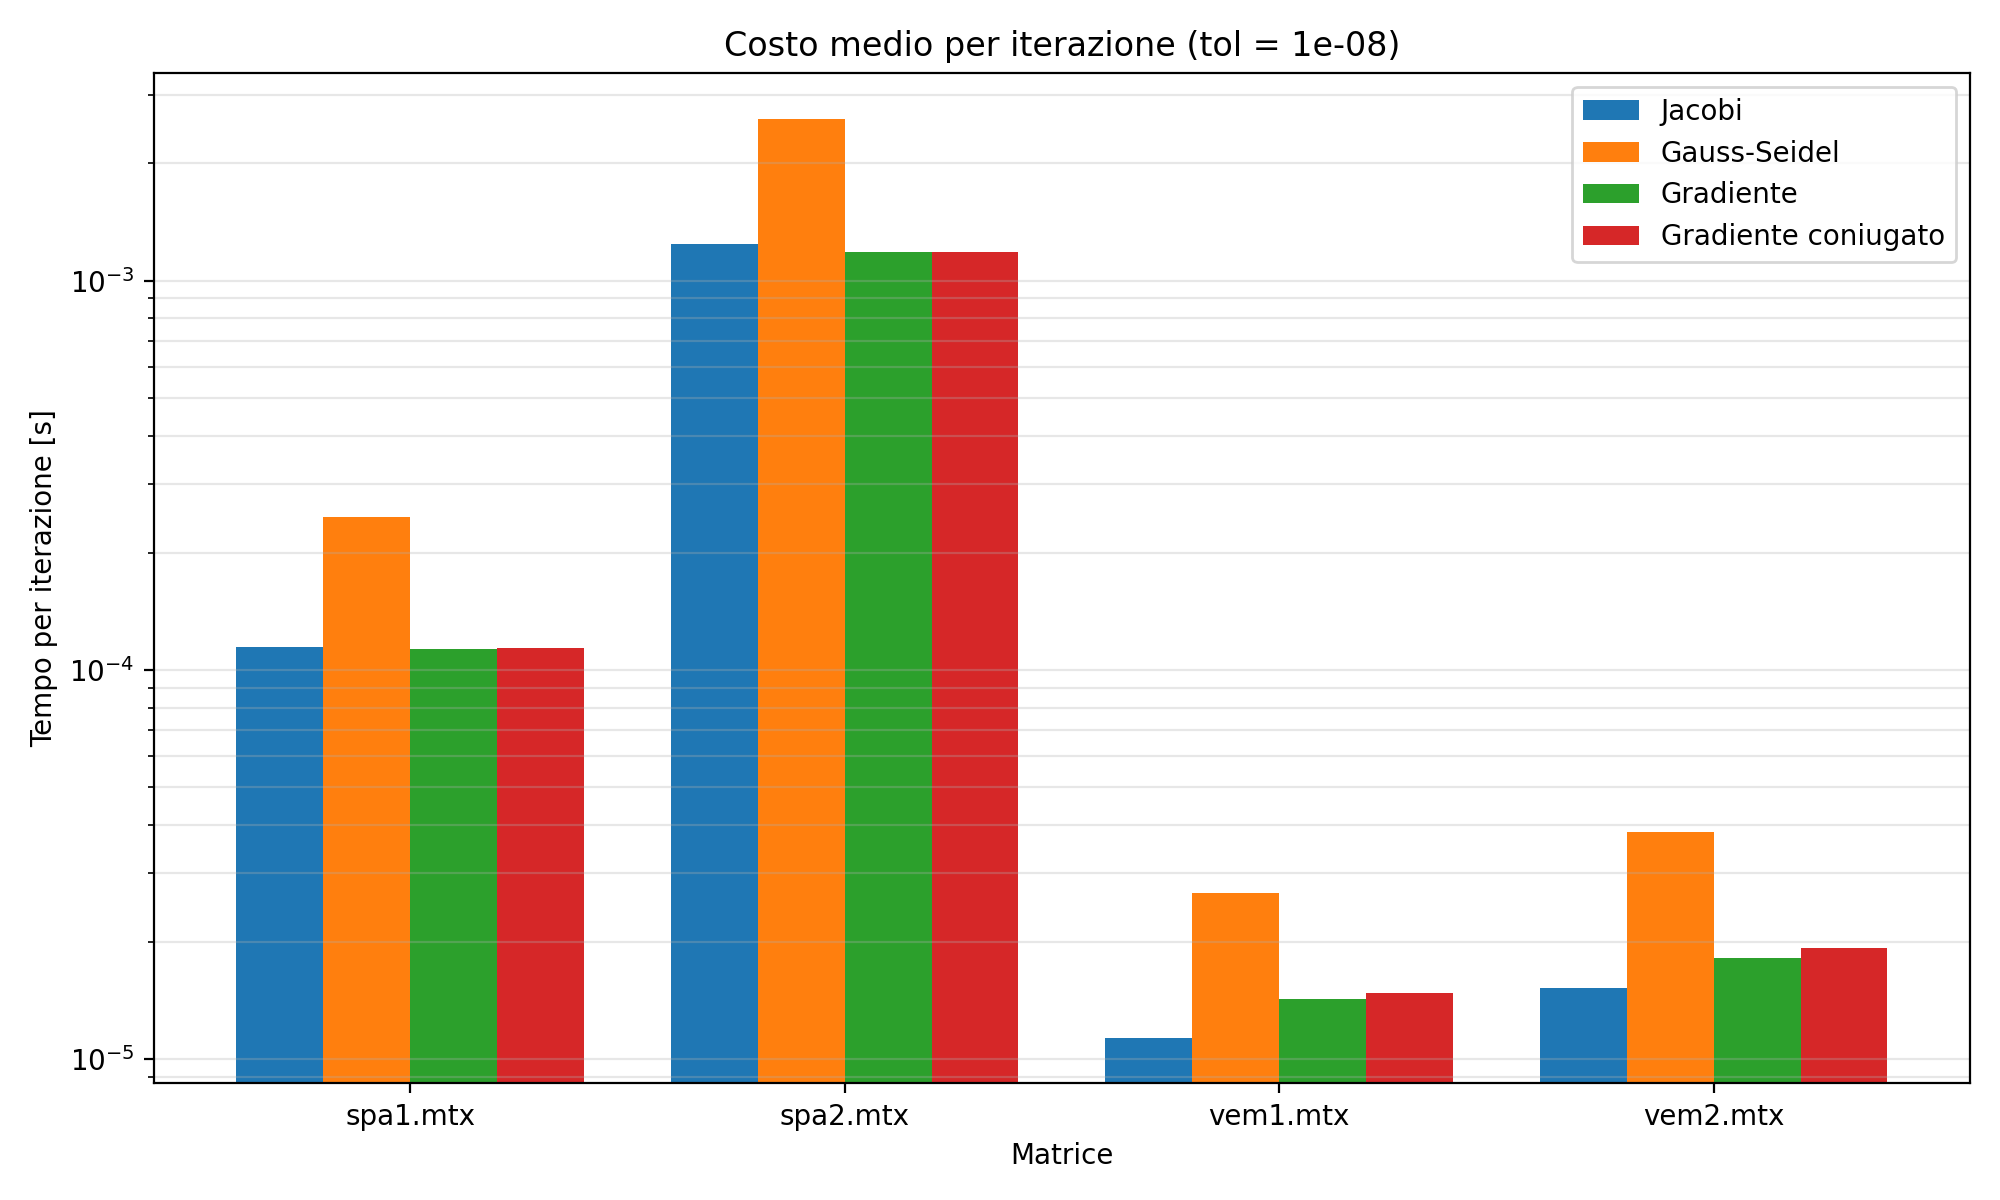
\includegraphics[width=0.78\textwidth]{../results/plots/cost_per_iter.png}
\caption{Costo medio per iterazione (\texttt{tol}$=10^{-8}$, asse $y$ logaritmico),
che isola il peso del singolo passo dal numero di passi.}
\label{fig:costiter}
\end{figure}

Avendo osservato divari di tempo anche di tre ordini di grandezza, la nostra
intuizione è che essi dipendano dal \emph{numero} di iterazioni più che dal costo
del singolo passo. Per isolare quest'ultimo abbiamo calcolato il tempo medio per
iterazione --- tempo totale diviso per il numero di passi --- riportato nella
Figura~\ref{fig:costiter}.

L'osservazione convalida la nostra intuizione. A parità di matrice il costo per
iterazione è sostanzialmente uniforme fra i metodi, con Gauss--Seidel circa il
doppio degli altri --- per via della \emph{sweep} sequenziale che si somma al
prodotto matrice--vettore --- e cresce con la densità della matrice, dall'ordine di
$10^{-5}$\,s sulle \texttt{vem} fino a $\sim$$10^{-3}$\,s su \texttt{spa2}, in linea
con il numero di non-zeri. Poiché il singolo passo costa più o meno lo stesso per
tutti, le enormi differenze di tempo totale viste in precedenza non nascono dal
costo dell'iterazione, ma dal loro \textbf{numero}. È questa la chiave di lettura
che tiene insieme tutti i grafici precedenti.

\clearpage
% ==================================================================
\section{Comparativa generale}
% ==================================================================
Mettendo a fattor comune le tre letture precedenti emerge un quadro coerente, che
si lascia riassumere in poche affermazioni.

\paragraph{Due leggi distinte per due famiglie di metodi.}
La velocità di Jacobi e Gauss--Seidel è governata dalla \textbf{dominanza
diagonale} della matrice, quella di Gradiente e Gradiente coniugato dal
\textbf{numero di condizionamento}. È questo il motivo per cui le stesse matrici
producono classifiche opposte: sulle \texttt{spa} (dominanti ma mal condizionate)
gli stazionari volano e il Gradiente arranca; sulle \texttt{vem} (poco dominanti
ma ben condizionate) accade il contrario.

\paragraph{Gauss--Seidel batte sistematicamente Jacobi.}
Riusando immediatamente le componenti appena calcolate, Gauss--Seidel dimezza con
regolarità le iterazioni di Jacobi (su \texttt{vem2} a $\texttt{tol}=10^{-8}$,
$2\,714$ contro $5\,425$). Il suo passo è però sequenziale e un po' più caro: sulle
\texttt{vem} molto sparse i tempi dei due si avvicinano, mentre sulle \texttt{spa},
dove converge in pochissimi passi, è nettamente il più rapido tra gli stazionari.

\paragraph{Il Gradiente coniugato è il vincitore in ogni scenario.}
Converge sempre in poche decine di iterazioni ($38$--$240$), con crescita
lentissima al ridursi di \texttt{tol}, segue da vicino la legge
$\propto\sqrt{\mathrm{cond}(A)}$ e resta sempre ben al di sotto del limite teorico
di $n$ passi. A parità di tolleranza restituisce inoltre l'errore più piccolo, e
sulle matrici dense è il più veloce dopo Gauss--Seidel, su quelle sparse il più
veloce in assoluto.

\paragraph{Il Gradiente semplice è il più fragile.}
La sua direzione di massima discesa, sulle matrici mal condizionate, innesca lo
\emph{zig-zag}: il numero di iterazioni cresce con $\mathrm{cond}(A)$ e, quando il
\emph{matvec} è costoso, il tempo degrada in modo severo. È competitivo solo dove
la matrice è ben condizionata.

\medskip
\noindent In sintesi, su questo insieme di prove il \textbf{Gradiente coniugato è
la scelta di riferimento}; tra i metodi stazionari, Gauss--Seidel domina Jacobi; il
Gradiente semplice va riservato ai casi ben condizionati. L'andamento sperimentale,
in ognuna delle tre metriche, rispetta le predizioni teoriche dei metodi.

\clearpage
% ==================================================================
\appendix
\section{Codice completo}
% ==================================================================
Si riporta di seguito il codice sorgente completo della libreria e degli script di
supporto. Il cuore dei solutori è \texttt{solvers.py}; \texttt{run\_assignment.py}
è l'eseguibile di validazione; \texttt{plots.py} produce sia i tre grafici
fondamentali della Sezione precedente sia i grafici di approfondimento;
\texttt{analyze\_cond.py} e \texttt{test\_assignment.py} sono gli strumenti a
contorno (condizionamento e test).

\subsection{\texttt{solvers.py}}
\lstinputlisting[style=pyfull]{../solvers.py}

\subsection{\texttt{run\_assignment.py}}
\lstinputlisting[style=pyfull]{../run_assignment.py}

\subsection{\texttt{plots.py}}
\lstinputlisting[style=pyfull]{../plots.py}

\subsection{\texttt{analyze\_cond.py}}
\lstinputlisting[style=pyfull]{../analyze_cond.py}

\subsection{\texttt{test\_assignment.py}}
\lstinputlisting[style=pyfull]{../test_assignment.py}

\end{document}
